\documentclass[1p]{elsarticle_modified}
%\bibliographystyle{elsarticle-num}

%\usepackage[colorlinks]{hyperref}
%\usepackage{abbrmath_seonhwa} %\Abb, \Ascr, \Acal ,\Abf, \Afrak
\usepackage{amsfonts}
\usepackage{amssymb}
\usepackage{amsmath}
\usepackage{amsthm}
\usepackage{scalefnt}
\usepackage{amsbsy}
\usepackage{kotex}
\usepackage{caption}
\usepackage{subfig}
\usepackage{color}
\usepackage{graphicx}
\usepackage{xcolor} %% white, black, red, green, blue, cyan, magenta, yellow
\usepackage{float}
\usepackage{setspace}
\usepackage{hyperref}

\usepackage{tikz}
\usetikzlibrary{arrows}

\usepackage{multirow}
\usepackage{array} % fixed length table
\usepackage{hhline}

%%%%%%%%%%%%%%%%%%%%%
\makeatletter
\renewcommand*\env@matrix[1][\arraystretch]{%
	\edef\arraystretch{#1}%
	\hskip -\arraycolsep
	\let\@ifnextchar\new@ifnextchar
	\array{*\c@MaxMatrixCols c}}
\makeatother %https://tex.stackexchange.com/questions/14071/how-can-i-increase-the-line-spacing-in-a-matrix
%%%%%%%%%%%%%%%

\usepackage[normalem]{ulem}

\newcommand{\msout}[1]{\ifmmode\text{\sout{\ensuremath{#1}}}\else\sout{#1}\fi}
%SOURCE: \msout is \stkout macro in https://tex.stackexchange.com/questions/20609/strikeout-in-math-mode

\newcommand{\cancel}[1]{
	\ifmmode
	{\color{red}\msout{#1}}
	\else
	{\color{red}\sout{#1}}
	\fi
}

\newcommand{\add}[1]{
	{\color{blue}\uwave{#1}}
}

\newcommand{\replace}[2]{
	\ifmmode
	{\color{red}\msout{#1}}{\color{blue}\uwave{#2}}
	\else
	{\color{red}\sout{#1}}{\color{blue}\uwave{#2}}
	\fi
}

\newcommand{\Sol}{\mathcal{S}} %segment
\newcommand{\D}{D} %diagram
\newcommand{\A}{\mathcal{A}} %arc


%%%%%%%%%%%%%%%%%%%%%%%%%%%%%5 test

\def\sl{\operatorname{\textup{SL}}(2,\Cbb)}
\def\psl{\operatorname{\textup{PSL}}(2,\Cbb)}
\def\quan{\mkern 1mu \triangleright \mkern 1mu}

\theoremstyle{definition}
\newtheorem{thm}{Theorem}[section]
\newtheorem{prop}[thm]{Proposition}
\newtheorem{lem}[thm]{Lemma}
\newtheorem{ques}[thm]{Question}
\newtheorem{cor}[thm]{Corollary}
\newtheorem{defn}[thm]{Definition}
\newtheorem{exam}[thm]{Example}
\newtheorem{rmk}[thm]{Remark}
\newtheorem{alg}[thm]{Algorithm}

\newcommand{\I}{\sqrt{-1}}
\begin{document}

%\begin{frontmatter}
%
%\title{Boundary parabolic representations of knots up to 8 crossings}
%
%%% Group authors per affiliation:
%\author{Yunhi Cho} 
%\address{Department of Mathematics, University of Seoul, Seoul, Korea}
%\ead{yhcho@uos.ac.kr}
%
%
%\author{Seonhwa Kim} %\fnref{s_kim}}
%\address{Center for Geometry and Physics, Institute for Basic Science, Pohang, 37673, Korea}
%\ead{ryeona17@ibs.re.kr}
%
%\author{Hyuk Kim}
%\address{Department of Mathematical Sciences, Seoul National University, Seoul 08826, Korea}
%\ead{hyukkim@snu.ac.kr}
%
%\author{Seokbeom Yoon}
%\address{Department of Mathematical Sciences, Seoul National University, Seoul, 08826,  Korea}
%\ead{sbyoon15@snu.ac.kr}
%
%\begin{abstract}
%We find all boundary parabolic representation of knots up to 8 crossings.
%
%\end{abstract}
%\begin{keyword}
%    \MSC[2010] 57M25 
%\end{keyword}
%
%\end{frontmatter}

%\linenumbers
%\tableofcontents
%
\newcommand\colored[1]{\textcolor{white}{\rule[-0.35ex]{0.8em}{1.4ex}}\kern-0.8em\color{red} #1}%
%\newcommand\colored[1]{\textcolor{white}{ #1}\kern-2.17ex	\textcolor{white}{ #1}\kern-1.81ex	\textcolor{white}{ #1}\kern-2.15ex\color{red}#1	}

{\Large $\underline{12a_{0903}~(K12a_{0903})}$}

\setlength{\tabcolsep}{10pt}
\renewcommand{\arraystretch}{1.6}
\vspace{1cm}\begin{tabular}{m{100pt}>{\centering\arraybackslash}m{274pt}}
\multirow{5}{120pt}{
	\centering
	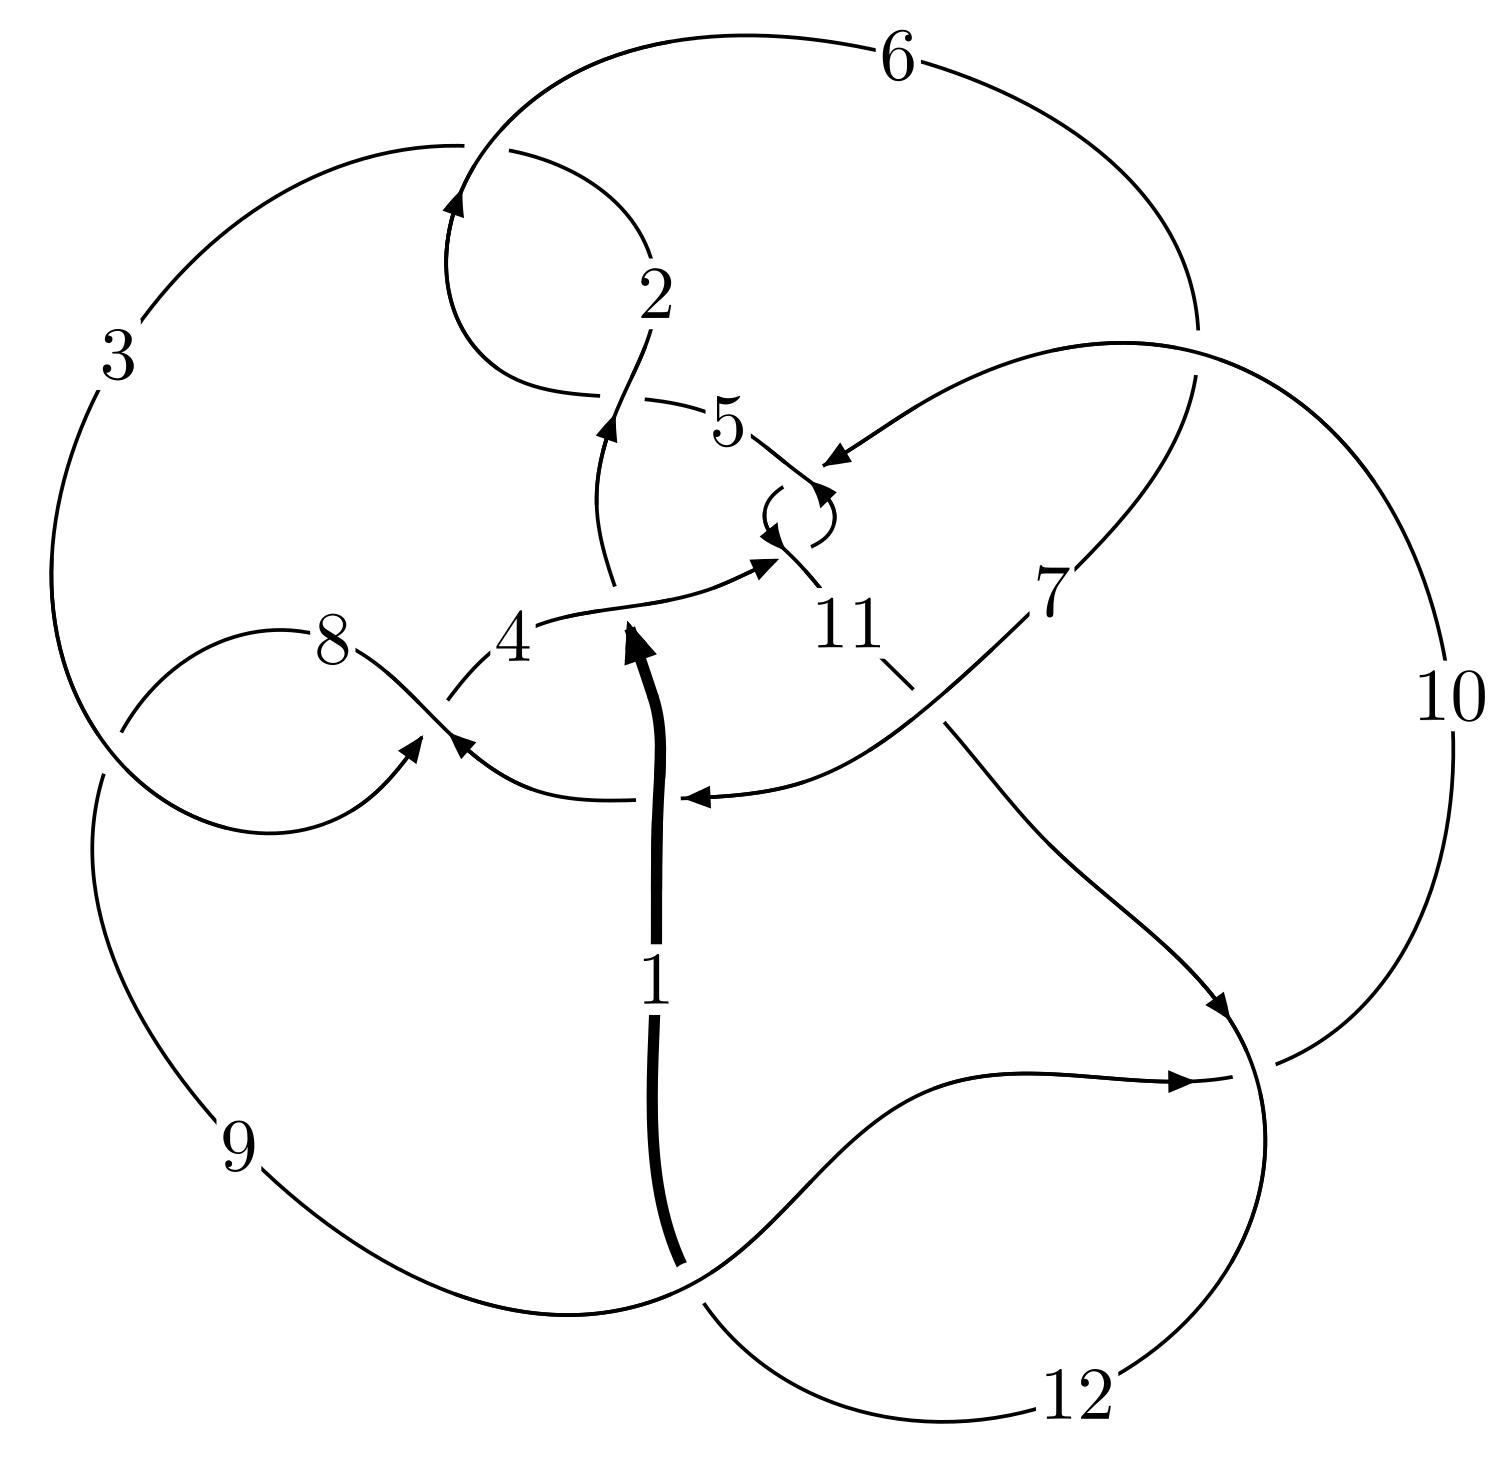
\includegraphics[width=112pt]{../../../GIT/diagram.site/Diagrams/png/1704_12a_0903.png}\\
\ \ \ A knot diagram\footnotemark}&
\allowdisplaybreaks
\textbf{Linearized knot diagam} \\
\cline{2-2}
 &
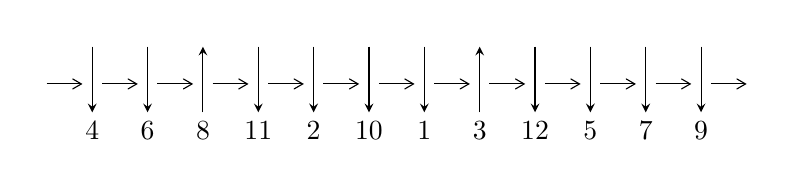
\begin{tikzpicture}[x=20pt, y=17pt]
	% nodes
	\node (C0) at (0, 0) {};
	\node (C1) at (1, 0) {};
	\node (C1U) at (1, +1) {};
	\node (C1D) at (1, -1) {4};

	\node (C2) at (2, 0) {};
	\node (C2U) at (2, +1) {};
	\node (C2D) at (2, -1) {6};

	\node (C3) at (3, 0) {};
	\node (C3U) at (3, +1) {};
	\node (C3D) at (3, -1) {8};

	\node (C4) at (4, 0) {};
	\node (C4U) at (4, +1) {};
	\node (C4D) at (4, -1) {11};

	\node (C5) at (5, 0) {};
	\node (C5U) at (5, +1) {};
	\node (C5D) at (5, -1) {2};

	\node (C6) at (6, 0) {};
	\node (C6U) at (6, +1) {};
	\node (C6D) at (6, -1) {10};

	\node (C7) at (7, 0) {};
	\node (C7U) at (7, +1) {};
	\node (C7D) at (7, -1) {1};

	\node (C8) at (8, 0) {};
	\node (C8U) at (8, +1) {};
	\node (C8D) at (8, -1) {3};

	\node (C9) at (9, 0) {};
	\node (C9U) at (9, +1) {};
	\node (C9D) at (9, -1) {12};

	\node (C10) at (10, 0) {};
	\node (C10U) at (10, +1) {};
	\node (C10D) at (10, -1) {5};

	\node (C11) at (11, 0) {};
	\node (C11U) at (11, +1) {};
	\node (C11D) at (11, -1) {7};

	\node (C12) at (12, 0) {};
	\node (C12U) at (12, +1) {};
	\node (C12D) at (12, -1) {9};
	\node (C13) at (13, 0) {};

	% arrows
	\draw[->,>={angle 60}]
	(C0) edge (C1) (C1) edge (C2) (C2) edge (C3) (C3) edge (C4) (C4) edge (C5) (C5) edge (C6) (C6) edge (C7) (C7) edge (C8) (C8) edge (C9) (C9) edge (C10) (C10) edge (C11) (C11) edge (C12) (C12) edge (C13) ;	\draw[->,>=stealth]
	(C1U) edge (C1D) (C2U) edge (C2D) (C3D) edge (C3U) (C4U) edge (C4D) (C5U) edge (C5D) (C6U) edge (C6D) (C7U) edge (C7D) (C8D) edge (C8U) (C9U) edge (C9D) (C10U) edge (C10D) (C11U) edge (C11D) (C12U) edge (C12D) ;
	\end{tikzpicture} \\
\hhline{~~} \\& 
\textbf{Solving Sequence} \\ \cline{2-2} 
 &
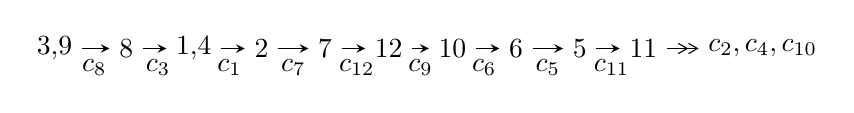
\begin{tikzpicture}[x=23pt, y=7pt]
	% node
	\node (A0) at (-1/8, 0) {3,9};
	\node (A1) at (1, 0) {8};
	\node (A2) at (33/16, 0) {1,4};
	\node (A3) at (25/8, 0) {2};
	\node (A4) at (33/8, 0) {7};
	\node (A5) at (41/8, 0) {12};
	\node (A6) at (49/8, 0) {10};
	\node (A7) at (57/8, 0) {6};
	\node (A8) at (65/8, 0) {5};
	\node (A9) at (73/8, 0) {11};
	\node (C1) at (1/2, -1) {$c_{8}$};
	\node (C2) at (3/2, -1) {$c_{3}$};
	\node (C3) at (21/8, -1) {$c_{1}$};
	\node (C4) at (29/8, -1) {$c_{7}$};
	\node (C5) at (37/8, -1) {$c_{12}$};
	\node (C6) at (45/8, -1) {$c_{9}$};
	\node (C7) at (53/8, -1) {$c_{6}$};
	\node (C8) at (61/8, -1) {$c_{5}$};
	\node (C9) at (69/8, -1) {$c_{11}$};
	\node (A10) at (11, 0) {$c_{2},c_{4},c_{10}$};

	% edge
	\draw[->,>=stealth]	
	(A0) edge (A1) (A1) edge (A2) (A2) edge (A3) (A3) edge (A4) (A4) edge (A5) (A5) edge (A6) (A6) edge (A7) (A7) edge (A8) (A8) edge (A9) ;
	\draw[->>,>={angle 60}]	
	(A9) edge (A10);
\end{tikzpicture} \\ 

\end{tabular} \\

\footnotetext{
The image of knot diagram is generated by the software ``\textbf{Draw programme}" developed by Andrew Bartholomew(\url{http://www.layer8.co.uk/maths/draw/index.htm\#Running-draw}), where we modified some parts for our purpose(\url{https://github.com/CATsTAILs/LinksPainter}).
}\phantom \\ \newline 
\centering \textbf{Ideals for irreducible components\footnotemark of $X_{\text{par}}$} 
 
\begin{align*}
I^u_{1}&=\langle 
6.28945\times10^{1064} u^{172}+1.31632\times10^{1064} u^{171}+\cdots+1.81307\times10^{1066} b-3.19196\times10^{1069},\\
\phantom{I^u_{1}}&\phantom{= \langle  }3.68475\times10^{1069} u^{172}+6.81125\times10^{1069} u^{171}+\cdots+1.07575\times10^{1071} a+1.11222\times10^{1074},\\
\phantom{I^u_{1}}&\phantom{= \langle  }u^{173}+u^{172}+\cdots+818273 u+59333\rangle \\
I^u_{2}&=\langle 
3.81902\times10^{35} u^{44}-2.24338\times10^{35} u^{43}+\cdots+3.19337\times10^{33} b-3.10619\times10^{35},\\
\phantom{I^u_{2}}&\phantom{= \langle  }-5.69864\times10^{35} u^{44}-7.52359\times10^{35} u^{43}+\cdots+3.19337\times10^{33} a-1.57081\times10^{36},\\
\phantom{I^u_{2}}&\phantom{= \langle  }u^{45}+18 u^{43}+\cdots+17 u^2+1\rangle \\
I^u_{3}&=\langle 
b,\;u^3- u^2+a+u,\;u^4+u^2+u+1\rangle \\
\\
\end{align*}
\raggedright * 3 irreducible components of $\dim_{\mathbb{C}}=0$, with total 222 representations.\\
\footnotetext{All coefficients of polynomials are rational numbers. But the coefficients are sometimes approximated in decimal forms when there is not enough margin.}
\newpage
\renewcommand{\arraystretch}{1}
\centering \section*{I. $I^u_{1}= \langle 6.29\times10^{1064} u^{172}+1.32\times10^{1064} u^{171}+\cdots+1.81\times10^{1066} b-3.19\times10^{1069},\;3.68\times10^{1069} u^{172}+6.81\times10^{1069} u^{171}+\cdots+1.08\times10^{1071} a+1.11\times10^{1074},\;u^{173}+u^{172}+\cdots+818273 u+59333 \rangle$}
\flushleft \textbf{(i) Arc colorings}\\
\begin{tabular}{m{7pt} m{180pt} m{7pt} m{180pt} }
\flushright $a_{3}=$&$\begin{pmatrix}0\\u\end{pmatrix}$ \\
\flushright $a_{9}=$&$\begin{pmatrix}1\\0\end{pmatrix}$ \\
\flushright $a_{8}=$&$\begin{pmatrix}1\\u^2\end{pmatrix}$ \\
\flushright $a_{1}=$&$\begin{pmatrix}-0.0342528 u^{172}-0.0633162 u^{171}+\cdots-15662.1 u-1033.90\\-0.0346895 u^{172}-0.00726018 u^{171}+\cdots+20161.3 u+1760.53\end{pmatrix}$ \\
\flushright $a_{4}=$&$\begin{pmatrix}u\\u^3+u\end{pmatrix}$ \\
\flushright $a_{2}=$&$\begin{pmatrix}-0.0477650 u^{172}-0.0456886 u^{171}+\cdots+10111.1 u+992.107\\-0.0442190 u^{172}-0.00774286 u^{171}+\cdots+21255.2 u+1938.91\end{pmatrix}$ \\
\flushright $a_{7}=$&$\begin{pmatrix}-0.0690865 u^{172}-0.132099 u^{171}+\cdots-88077.9 u-6249.36\\0.0291113 u^{172}+0.00918828 u^{171}+\cdots-5126.00 u-626.952\end{pmatrix}$ \\
\flushright $a_{12}=$&$\begin{pmatrix}-0.0689423 u^{172}-0.0705764 u^{171}+\cdots+4499.15 u+726.629\\-0.0346895 u^{172}-0.00726018 u^{171}+\cdots+20161.3 u+1760.53\end{pmatrix}$ \\
\flushright $a_{10}=$&$\begin{pmatrix}-0.0189660 u^{172}+0.0100952 u^{171}+\cdots+34750.5 u+2620.23\\-0.0388657 u^{172}-0.00861547 u^{171}+\cdots+4918.24 u+697.500\end{pmatrix}$ \\
\flushright $a_{6}=$&$\begin{pmatrix}0.0402518 u^{172}+0.00362436 u^{171}+\cdots-27493.3 u-2377.65\\0.109608 u^{172}+0.0254614 u^{171}+\cdots-91115.0 u-7455.54\end{pmatrix}$ \\
\flushright $a_{5}=$&$\begin{pmatrix}0.0427315 u^{172}-0.0298589 u^{171}+\cdots-92111.9 u-7144.99\\0.0766791 u^{172}-0.0138396 u^{171}+\cdots-86901.4 u-6811.41\end{pmatrix}$ \\
\flushright $a_{11}=$&$\begin{pmatrix}0.100360 u^{172}+0.0919849 u^{171}+\cdots+27574.0 u+1302.19\\0.0174467 u^{172}-0.0184323 u^{171}+\cdots-59319.7 u-4407.27\end{pmatrix}$\\&\end{tabular}
\flushleft \textbf{(ii) Obstruction class $= -1$}\\~\\
\flushleft \textbf{(iii) Cusp Shapes $= -0.354297 u^{172}-0.576879 u^{171}+\cdots-512725. u-34786.1$}\\~\\
\newpage\renewcommand{\arraystretch}{1}
\flushleft \textbf{(iv) u-Polynomials at the component}\newline \\
\begin{tabular}{m{50pt}|m{274pt}}
Crossings & \hspace{64pt}u-Polynomials at each crossing \\
\hline $$\begin{aligned}c_{1}\end{aligned}$$&$\begin{aligned}
&u^{173}-5 u^{172}+\cdots+34978845458 u-5461860410
\end{aligned}$\\
\hline $$\begin{aligned}c_{2},c_{5}\end{aligned}$$&$\begin{aligned}
&u^{173}+4 u^{172}+\cdots+7855501 u+378351
\end{aligned}$\\
\hline $$\begin{aligned}c_{3},c_{8}\end{aligned}$$&$\begin{aligned}
&u^{173}+u^{172}+\cdots+818273 u+59333
\end{aligned}$\\
\hline $$\begin{aligned}c_{4},c_{10}\end{aligned}$$&$\begin{aligned}
&u^{173}- u^{172}+\cdots+4515 u+3617
\end{aligned}$\\
\hline $$\begin{aligned}c_{6}\end{aligned}$$&$\begin{aligned}
&u^{173}+8 u^{172}+\cdots+725366244 u+32903701
\end{aligned}$\\
\hline $$\begin{aligned}c_{7}\end{aligned}$$&$\begin{aligned}
&u^{173}+2 u^{172}+\cdots+127844 u+7121
\end{aligned}$\\
\hline $$\begin{aligned}c_{9},c_{12}\end{aligned}$$&$\begin{aligned}
&u^{173}-8 u^{172}+\cdots-1082392 u+116112
\end{aligned}$\\
\hline $$\begin{aligned}c_{11}\end{aligned}$$&$\begin{aligned}
&u^{173}+10 u^{172}+\cdots+22516 u+5257
\end{aligned}$\\
\hline
\end{tabular}\\~\\
\newpage\renewcommand{\arraystretch}{1}
\flushleft \textbf{(v) Riley Polynomials at the component}\newline \\
\begin{tabular}{m{50pt}|m{274pt}}
Crossings & \hspace{64pt}Riley Polynomials at each crossing \\
\hline $$\begin{aligned}c_{1}\end{aligned}$$&$\begin{aligned}
&y^{173}-57 y^{172}+\cdots+1.76\times10^{21} y-2.98\times10^{19}
\end{aligned}$\\
\hline $$\begin{aligned}c_{2},c_{5}\end{aligned}$$&$\begin{aligned}
&y^{173}-84 y^{172}+\cdots+18389284184671 y-143149479201
\end{aligned}$\\
\hline $$\begin{aligned}c_{3},c_{8}\end{aligned}$$&$\begin{aligned}
&y^{173}+111 y^{172}+\cdots-76077907077 y-3520404889
\end{aligned}$\\
\hline $$\begin{aligned}c_{4},c_{10}\end{aligned}$$&$\begin{aligned}
&y^{173}+97 y^{172}+\cdots-638718983 y-13082689
\end{aligned}$\\
\hline $$\begin{aligned}c_{6}\end{aligned}$$&$\begin{aligned}
&y^{173}+38 y^{172}+\cdots+138215553352212392 y-1082653539497401
\end{aligned}$\\
\hline $$\begin{aligned}c_{7}\end{aligned}$$&$\begin{aligned}
&y^{173}-4 y^{172}+\cdots-4733202902 y-50708641
\end{aligned}$\\
\hline $$\begin{aligned}c_{9},c_{12}\end{aligned}$$&$\begin{aligned}
&y^{173}+120 y^{172}+\cdots-719338416320 y-13481996544
\end{aligned}$\\
\hline $$\begin{aligned}c_{11}\end{aligned}$$&$\begin{aligned}
&y^{173}+4 y^{172}+\cdots-148893064 y-27636049
\end{aligned}$\\
\hline
\end{tabular}\\~\\
\newpage\flushleft \textbf{(vi) Complex Volumes and Cusp Shapes}
$$\begin{array}{c|c|c}  
\text{Solutions to }I^u_{1}& \I (\text{vol} + \sqrt{-1}CS) & \text{Cusp shape}\\
 \hline 
\begin{aligned}
u &= -0.200695 + 0.983674 I \\
a &= \phantom{-}0.099596 - 1.101180 I \\
b &= -0.300391 + 0.865055 I\end{aligned}
 & -1.14533 + 1.31544 I & \phantom{-0.000000 } 0 \\ \hline\begin{aligned}
u &= -0.200695 - 0.983674 I \\
a &= \phantom{-}0.099596 + 1.101180 I \\
b &= -0.300391 - 0.865055 I\end{aligned}
 & -1.14533 - 1.31544 I & \phantom{-0.000000 } 0 \\ \hline\begin{aligned}
u &= \phantom{-}0.238962 + 0.976771 I \\
a &= -0.85300 - 1.75553 I \\
b &= \phantom{-}0.166763 - 1.275220 I\end{aligned}
 & \phantom{-}1.45317 + 9.45174 I & \phantom{-0.000000 } 0 \\ \hline\begin{aligned}
u &= \phantom{-}0.238962 - 0.976771 I \\
a &= -0.85300 + 1.75553 I \\
b &= \phantom{-}0.166763 + 1.275220 I\end{aligned}
 & \phantom{-}1.45317 - 9.45174 I & \phantom{-0.000000 } 0 \\ \hline\begin{aligned}
u &= \phantom{-}0.310932 + 0.937146 I \\
a &= -0.266639 - 1.322090 I \\
b &= \phantom{-}0.76410 + 1.60099 I\end{aligned}
 & \phantom{-}2.30031 + 1.47617 I & \phantom{-0.000000 } 0 \\ \hline\begin{aligned}
u &= \phantom{-}0.310932 - 0.937146 I \\
a &= -0.266639 + 1.322090 I \\
b &= \phantom{-}0.76410 - 1.60099 I\end{aligned}
 & \phantom{-}2.30031 - 1.47617 I & \phantom{-0.000000 } 0 \\ \hline\begin{aligned}
u &= \phantom{-}0.422422 + 0.944303 I \\
a &= -1.75931 - 1.00821 I \\
b &= \phantom{-}0.251193 - 1.248970 I\end{aligned}
 & \phantom{-}2.98127 + 3.28924 I & \phantom{-0.000000 } 0 \\ \hline\begin{aligned}
u &= \phantom{-}0.422422 - 0.944303 I \\
a &= -1.75931 + 1.00821 I \\
b &= \phantom{-}0.251193 + 1.248970 I\end{aligned}
 & \phantom{-}2.98127 - 3.28924 I & \phantom{-0.000000 } 0 \\ \hline\begin{aligned}
u &= \phantom{-}1.001610 + 0.259760 I \\
a &= -0.234073 - 0.456409 I \\
b &= -0.772152 - 0.286782 I\end{aligned}
 & -2.54970 + 2.40971 I & \phantom{-0.000000 } 0 \\ \hline\begin{aligned}
u &= \phantom{-}1.001610 - 0.259760 I \\
a &= -0.234073 + 0.456409 I \\
b &= -0.772152 + 0.286782 I\end{aligned}
 & -2.54970 - 2.40971 I & \phantom{-0.000000 } 0\\
 \hline 
 \end{array}$$\newpage$$\begin{array}{c|c|c}  
\text{Solutions to }I^u_{1}& \I (\text{vol} + \sqrt{-1}CS) & \text{Cusp shape}\\
 \hline 
\begin{aligned}
u &= \phantom{-}0.644326 + 0.717506 I \\
a &= -0.196592 - 0.236738 I \\
b &= \phantom{-}0.48186 + 1.36306 I\end{aligned}
 & \phantom{-}4.48340 - 5.92423 I & \phantom{-0.000000 } 0 \\ \hline\begin{aligned}
u &= \phantom{-}0.644326 - 0.717506 I \\
a &= -0.196592 + 0.236738 I \\
b &= \phantom{-}0.48186 - 1.36306 I\end{aligned}
 & \phantom{-}4.48340 + 5.92423 I & \phantom{-0.000000 } 0 \\ \hline\begin{aligned}
u &= -0.960899 + 0.053428 I \\
a &= -0.573354 - 0.300532 I \\
b &= \phantom{-}0.133195 - 0.911360 I\end{aligned}
 & -1.48764 + 1.19567 I & \phantom{-0.000000 } 0 \\ \hline\begin{aligned}
u &= -0.960899 - 0.053428 I \\
a &= -0.573354 + 0.300532 I \\
b &= \phantom{-}0.133195 + 0.911360 I\end{aligned}
 & -1.48764 - 1.19567 I & \phantom{-0.000000 } 0 \\ \hline\begin{aligned}
u &= -0.422732 + 0.858394 I \\
a &= \phantom{-}2.59637 - 0.57540 I \\
b &= -0.070848 - 1.196950 I\end{aligned}
 & \phantom{-}3.46056 - 6.65815 I & \phantom{-0.000000 } 0 \\ \hline\begin{aligned}
u &= -0.422732 - 0.858394 I \\
a &= \phantom{-}2.59637 + 0.57540 I \\
b &= -0.070848 + 1.196950 I\end{aligned}
 & \phantom{-}3.46056 + 6.65815 I & \phantom{-0.000000 } 0 \\ \hline\begin{aligned}
u &= \phantom{-}0.538570 + 0.895585 I \\
a &= -2.20809 + 0.16514 I \\
b &= \phantom{-}0.68648 - 1.23900 I\end{aligned}
 & \phantom{-}3.93045 + 10.55550 I & \phantom{-0.000000 } 0 \\ \hline\begin{aligned}
u &= \phantom{-}0.538570 - 0.895585 I \\
a &= -2.20809 - 0.16514 I \\
b &= \phantom{-}0.68648 + 1.23900 I\end{aligned}
 & \phantom{-}3.93045 - 10.55550 I & \phantom{-0.000000 } 0 \\ \hline\begin{aligned}
u &= \phantom{-}0.123622 + 0.946070 I \\
a &= -0.413155 + 0.378308 I \\
b &= -0.10101 - 1.69525 I\end{aligned}
 & -0.063851 - 0.587563 I & \phantom{-0.000000 } 0 \\ \hline\begin{aligned}
u &= \phantom{-}0.123622 - 0.946070 I \\
a &= -0.413155 - 0.378308 I \\
b &= -0.10101 + 1.69525 I\end{aligned}
 & -0.063851 + 0.587563 I & \phantom{-0.000000 } 0\\
 \hline 
 \end{array}$$\newpage$$\begin{array}{c|c|c}  
\text{Solutions to }I^u_{1}& \I (\text{vol} + \sqrt{-1}CS) & \text{Cusp shape}\\
 \hline 
\begin{aligned}
u &= -0.260715 + 1.013100 I \\
a &= \phantom{-}0.112130 + 1.016630 I \\
b &= \phantom{-}0.42334 - 1.92998 I\end{aligned}
 & \phantom{-}1.40101 - 6.53069 I & \phantom{-0.000000 } 0 \\ \hline\begin{aligned}
u &= -0.260715 - 1.013100 I \\
a &= \phantom{-}0.112130 - 1.016630 I \\
b &= \phantom{-}0.42334 + 1.92998 I\end{aligned}
 & \phantom{-}1.40101 + 6.53069 I & \phantom{-0.000000 } 0 \\ \hline\begin{aligned}
u &= -0.484556 + 0.937692 I \\
a &= \phantom{-}1.25963 - 1.03608 I \\
b &= -0.829834 + 0.213422 I\end{aligned}
 & -2.59855 - 2.68466 I & \phantom{-0.000000 } 0 \\ \hline\begin{aligned}
u &= -0.484556 - 0.937692 I \\
a &= \phantom{-}1.25963 + 1.03608 I \\
b &= -0.829834 - 0.213422 I\end{aligned}
 & -2.59855 + 2.68466 I & \phantom{-0.000000 } 0 \\ \hline\begin{aligned}
u &= -0.241499 + 1.030300 I \\
a &= \phantom{-}2.18143 + 1.49276 I \\
b &= -0.040701 - 1.056610 I\end{aligned}
 & \phantom{-}4.74593 + 0.10675 I & \phantom{-0.000000 } 0 \\ \hline\begin{aligned}
u &= -0.241499 - 1.030300 I \\
a &= \phantom{-}2.18143 - 1.49276 I \\
b &= -0.040701 + 1.056610 I\end{aligned}
 & \phantom{-}4.74593 - 0.10675 I & \phantom{-0.000000 } 0 \\ \hline\begin{aligned}
u &= -0.940511 + 0.041481 I \\
a &= -0.054074 - 0.608164 I \\
b &= \phantom{-}0.851988 - 0.060783 I\end{aligned}
 & -0.22897 - 9.03529 I & \phantom{-0.000000 } 0 \\ \hline\begin{aligned}
u &= -0.940511 - 0.041481 I \\
a &= -0.054074 + 0.608164 I \\
b &= \phantom{-}0.851988 + 0.060783 I\end{aligned}
 & -0.22897 + 9.03529 I & \phantom{-0.000000 } 0 \\ \hline\begin{aligned}
u &= -0.320339 + 1.010070 I \\
a &= \phantom{-}1.94948 + 0.50565 I \\
b &= -0.69852 - 1.53386 I\end{aligned}
 & -0.27735 - 7.08476 I & \phantom{-0.000000 } 0 \\ \hline\begin{aligned}
u &= -0.320339 - 1.010070 I \\
a &= \phantom{-}1.94948 - 0.50565 I \\
b &= -0.69852 + 1.53386 I\end{aligned}
 & -0.27735 + 7.08476 I & \phantom{-0.000000 } 0\\
 \hline 
 \end{array}$$\newpage$$\begin{array}{c|c|c}  
\text{Solutions to }I^u_{1}& \I (\text{vol} + \sqrt{-1}CS) & \text{Cusp shape}\\
 \hline 
\begin{aligned}
u &= \phantom{-}0.168961 + 0.922551 I \\
a &= \phantom{-}1.75791 - 1.25810 I \\
b &= -0.54516 + 1.34894 I\end{aligned}
 & -0.12681 + 1.91606 I & \phantom{-0.000000 } 0 \\ \hline\begin{aligned}
u &= \phantom{-}0.168961 - 0.922551 I \\
a &= \phantom{-}1.75791 + 1.25810 I \\
b &= -0.54516 - 1.34894 I\end{aligned}
 & -0.12681 - 1.91606 I & \phantom{-0.000000 } 0 \\ \hline\begin{aligned}
u &= -0.179170 + 0.916415 I \\
a &= \phantom{-}0.527452 - 1.173700 I \\
b &= -0.173887 - 1.340160 I\end{aligned}
 & -0.26861 - 4.57877 I & \phantom{-0.000000 } 0 \\ \hline\begin{aligned}
u &= -0.179170 - 0.916415 I \\
a &= \phantom{-}0.527452 + 1.173700 I \\
b &= -0.173887 + 1.340160 I\end{aligned}
 & -0.26861 + 4.57877 I & \phantom{-0.000000 } 0 \\ \hline\begin{aligned}
u &= \phantom{-}1.065240 + 0.105937 I \\
a &= -0.264381 + 0.425510 I \\
b &= \phantom{-}0.332949 + 1.307200 I\end{aligned}
 & \phantom{-}6.92967 - 7.56473 I & \phantom{-0.000000 } 0 \\ \hline\begin{aligned}
u &= \phantom{-}1.065240 - 0.105937 I \\
a &= -0.264381 - 0.425510 I \\
b &= \phantom{-}0.332949 - 1.307200 I\end{aligned}
 & \phantom{-}6.92967 + 7.56473 I & \phantom{-0.000000 } 0 \\ \hline\begin{aligned}
u &= -0.334971 + 1.021610 I \\
a &= -1.71258 - 0.81682 I \\
b &= \phantom{-}0.63493 + 1.27867 I\end{aligned}
 & \phantom{-}5.54370 - 6.15762 I & \phantom{-0.000000 } 0 \\ \hline\begin{aligned}
u &= -0.334971 - 1.021610 I \\
a &= -1.71258 + 0.81682 I \\
b &= \phantom{-}0.63493 - 1.27867 I\end{aligned}
 & \phantom{-}5.54370 + 6.15762 I & \phantom{-0.000000 } 0 \\ \hline\begin{aligned}
u &= -0.613604 + 0.689976 I \\
a &= \phantom{-}1.212130 - 0.573384 I \\
b &= -0.343083 - 1.275000 I\end{aligned}
 & \phantom{-}2.48008 - 5.65404 I & \phantom{-0.000000 } 0 \\ \hline\begin{aligned}
u &= -0.613604 - 0.689976 I \\
a &= \phantom{-}1.212130 + 0.573384 I \\
b &= -0.343083 + 1.275000 I\end{aligned}
 & \phantom{-}2.48008 + 5.65404 I & \phantom{-0.000000 } 0\\
 \hline 
 \end{array}$$\newpage$$\begin{array}{c|c|c}  
\text{Solutions to }I^u_{1}& \I (\text{vol} + \sqrt{-1}CS) & \text{Cusp shape}\\
 \hline 
\begin{aligned}
u &= -0.855720 + 0.326054 I \\
a &= \phantom{-}0.026482 + 0.562497 I \\
b &= -0.345573 + 1.304350 I\end{aligned}
 & \phantom{-}3.32095 + 3.55947 I & \phantom{-0.000000 } 0 \\ \hline\begin{aligned}
u &= -0.855720 - 0.326054 I \\
a &= \phantom{-}0.026482 - 0.562497 I \\
b &= -0.345573 - 1.304350 I\end{aligned}
 & \phantom{-}3.32095 - 3.55947 I & \phantom{-0.000000 } 0 \\ \hline\begin{aligned}
u &= \phantom{-}0.498419 + 0.974019 I \\
a &= -1.148720 - 0.460274 I \\
b &= \phantom{-}1.052800 + 0.012207 I\end{aligned}
 & \phantom{-}0.074828 - 0.437307 I & \phantom{-0.000000 } 0 \\ \hline\begin{aligned}
u &= \phantom{-}0.498419 - 0.974019 I \\
a &= -1.148720 + 0.460274 I \\
b &= \phantom{-}1.052800 - 0.012207 I\end{aligned}
 & \phantom{-}0.074828 + 0.437307 I & \phantom{-0.000000 } 0 \\ \hline\begin{aligned}
u &= -0.853207 + 0.703439 I \\
a &= \phantom{-}0.441272 - 1.151180 I \\
b &= -0.003260 - 0.896503 I\end{aligned}
 & -2.17995 - 0.03180 I & \phantom{-0.000000 } 0 \\ \hline\begin{aligned}
u &= -0.853207 - 0.703439 I \\
a &= \phantom{-}0.441272 + 1.151180 I \\
b &= -0.003260 + 0.896503 I\end{aligned}
 & -2.17995 + 0.03180 I & \phantom{-0.000000 } 0 \\ \hline\begin{aligned}
u &= \phantom{-}0.435294 + 1.025140 I \\
a &= -1.80123 + 0.22678 I \\
b &= \phantom{-}0.134550 - 1.053260 I\end{aligned}
 & \phantom{-}1.51146 + 2.82649 I & \phantom{-0.000000 } 0 \\ \hline\begin{aligned}
u &= \phantom{-}0.435294 - 1.025140 I \\
a &= -1.80123 - 0.22678 I \\
b &= \phantom{-}0.134550 + 1.053260 I\end{aligned}
 & \phantom{-}1.51146 - 2.82649 I & \phantom{-0.000000 } 0 \\ \hline\begin{aligned}
u &= \phantom{-}0.670930 + 0.899795 I \\
a &= -1.45134 - 0.83472 I \\
b &= \phantom{-}0.028957 - 0.888822 I\end{aligned}
 & -0.97851 + 4.44415 I & \phantom{-0.000000 } 0 \\ \hline\begin{aligned}
u &= \phantom{-}0.670930 - 0.899795 I \\
a &= -1.45134 + 0.83472 I \\
b &= \phantom{-}0.028957 + 0.888822 I\end{aligned}
 & -0.97851 - 4.44415 I & \phantom{-0.000000 } 0\\
 \hline 
 \end{array}$$\newpage$$\begin{array}{c|c|c}  
\text{Solutions to }I^u_{1}& \I (\text{vol} + \sqrt{-1}CS) & \text{Cusp shape}\\
 \hline 
\begin{aligned}
u &= \phantom{-}0.207523 + 0.844878 I \\
a &= -0.736815 - 0.346037 I \\
b &= \phantom{-}0.218523 + 0.270180 I\end{aligned}
 & -0.614594 + 1.120450 I & \phantom{-0.000000 } 0 \\ \hline\begin{aligned}
u &= \phantom{-}0.207523 - 0.844878 I \\
a &= -0.736815 + 0.346037 I \\
b &= \phantom{-}0.218523 - 0.270180 I\end{aligned}
 & -0.614594 - 1.120450 I & \phantom{-0.000000 } 0 \\ \hline\begin{aligned}
u &= -0.085049 + 0.861726 I \\
a &= -0.27790 + 2.38839 I \\
b &= \phantom{-}0.012082 + 1.306460 I\end{aligned}
 & \phantom{-}5.73234 - 1.49184 I & \phantom{-0.000000 } 0 \\ \hline\begin{aligned}
u &= -0.085049 - 0.861726 I \\
a &= -0.27790 - 2.38839 I \\
b &= \phantom{-}0.012082 - 1.306460 I\end{aligned}
 & \phantom{-}5.73234 + 1.49184 I & \phantom{-0.000000 } 0 \\ \hline\begin{aligned}
u &= \phantom{-}0.356815 + 1.077960 I \\
a &= \phantom{-}1.37784 + 0.60863 I \\
b &= -0.754663 - 0.739240 I\end{aligned}
 & -3.80490 + 5.05102 I & \phantom{-0.000000 } 0 \\ \hline\begin{aligned}
u &= \phantom{-}0.356815 - 1.077960 I \\
a &= \phantom{-}1.37784 - 0.60863 I \\
b &= -0.754663 + 0.739240 I\end{aligned}
 & -3.80490 - 5.05102 I & \phantom{-0.000000 } 0 \\ \hline\begin{aligned}
u &= -0.246800 + 0.818439 I \\
a &= -2.16972 - 1.12059 I \\
b &= -0.122048 + 0.942351 I\end{aligned}
 & -0.15321 + 2.55823 I & \phantom{-0.000000 } 0 \\ \hline\begin{aligned}
u &= -0.246800 - 0.818439 I \\
a &= -2.16972 + 1.12059 I \\
b &= -0.122048 - 0.942351 I\end{aligned}
 & -0.15321 - 2.55823 I & \phantom{-0.000000 } 0 \\ \hline\begin{aligned}
u &= -0.530803 + 0.669522 I \\
a &= -0.343924 + 1.198740 I \\
b &= -0.097619 + 1.346350 I\end{aligned}
 & \phantom{-}3.94899 + 2.73718 I & \phantom{-0.000000 } 0 \\ \hline\begin{aligned}
u &= -0.530803 - 0.669522 I \\
a &= -0.343924 - 1.198740 I \\
b &= -0.097619 - 1.346350 I\end{aligned}
 & \phantom{-}3.94899 - 2.73718 I & \phantom{-0.000000 } 0\\
 \hline 
 \end{array}$$\newpage$$\begin{array}{c|c|c}  
\text{Solutions to }I^u_{1}& \I (\text{vol} + \sqrt{-1}CS) & \text{Cusp shape}\\
 \hline 
\begin{aligned}
u &= \phantom{-}0.409556 + 1.087370 I \\
a &= -0.939268 - 0.715361 I \\
b &= \phantom{-}0.599246 + 0.029607 I\end{aligned}
 & -0.901550 + 0.201664 I & \phantom{-0.000000 } 0 \\ \hline\begin{aligned}
u &= \phantom{-}0.409556 - 1.087370 I \\
a &= -0.939268 + 0.715361 I \\
b &= \phantom{-}0.599246 - 0.029607 I\end{aligned}
 & -0.901550 - 0.201664 I & \phantom{-0.000000 } 0 \\ \hline\begin{aligned}
u &= -0.660910 + 0.498160 I \\
a &= \phantom{-}0.076156 + 0.293628 I \\
b &= -0.405297 + 1.312040 I\end{aligned}
 & \phantom{-}2.58653 + 3.21002 I & \phantom{-0.000000 } 0 \\ \hline\begin{aligned}
u &= -0.660910 - 0.498160 I \\
a &= \phantom{-}0.076156 - 0.293628 I \\
b &= -0.405297 - 1.312040 I\end{aligned}
 & \phantom{-}2.58653 - 3.21002 I & \phantom{-0.000000 } 0 \\ \hline\begin{aligned}
u &= -0.824688 + 0.041380 I \\
a &= \phantom{-}0.350309 - 0.198605 I \\
b &= \phantom{-}0.238297 - 1.284210 I\end{aligned}
 & \phantom{-}8.72034 + 2.85639 I & \phantom{-0.000000 } 0 \\ \hline\begin{aligned}
u &= -0.824688 - 0.041380 I \\
a &= \phantom{-}0.350309 + 0.198605 I \\
b &= \phantom{-}0.238297 + 1.284210 I\end{aligned}
 & \phantom{-}8.72034 - 2.85639 I & \phantom{-0.000000 } 0 \\ \hline\begin{aligned}
u &= -0.338746 + 1.124780 I \\
a &= \phantom{-}1.46946 - 0.46557 I \\
b &= -1.025100 - 0.095171 I\end{aligned}
 & -4.00976 - 3.22158 I & \phantom{-0.000000 } 0 \\ \hline\begin{aligned}
u &= -0.338746 - 1.124780 I \\
a &= \phantom{-}1.46946 + 0.46557 I \\
b &= -1.025100 + 0.095171 I\end{aligned}
 & -4.00976 + 3.22158 I & \phantom{-0.000000 } 0 \\ \hline\begin{aligned}
u &= \phantom{-}0.209148 + 0.788172 I \\
a &= \phantom{-}3.54030 - 1.24576 I \\
b &= \phantom{-}0.100915 + 0.957619 I\end{aligned}
 & \phantom{-}2.13521 - 7.36293 I & \phantom{-0.000000 } 0 \\ \hline\begin{aligned}
u &= \phantom{-}0.209148 - 0.788172 I \\
a &= \phantom{-}3.54030 + 1.24576 I \\
b &= \phantom{-}0.100915 - 0.957619 I\end{aligned}
 & \phantom{-}2.13521 + 7.36293 I & \phantom{-0.000000 } 0\\
 \hline 
 \end{array}$$\newpage$$\begin{array}{c|c|c}  
\text{Solutions to }I^u_{1}& \I (\text{vol} + \sqrt{-1}CS) & \text{Cusp shape}\\
 \hline 
\begin{aligned}
u &= \phantom{-}0.127461 + 0.793359 I \\
a &= -2.62023 + 0.52773 I \\
b &= \phantom{-}1.31779 - 0.97993 I\end{aligned}
 & \phantom{-}3.15145 + 0.80560 I & \phantom{-0.000000 } 0 \\ \hline\begin{aligned}
u &= \phantom{-}0.127461 - 0.793359 I \\
a &= -2.62023 - 0.52773 I \\
b &= \phantom{-}1.31779 + 0.97993 I\end{aligned}
 & \phantom{-}3.15145 - 0.80560 I & \phantom{-0.000000 } 0 \\ \hline\begin{aligned}
u &= -0.557566 + 1.061750 I \\
a &= \phantom{-}2.01247 - 0.01070 I \\
b &= -0.54909 - 1.30517 I\end{aligned}
 & \phantom{-}0.87998 - 7.95213 I & \phantom{-0.000000 } 0 \\ \hline\begin{aligned}
u &= -0.557566 - 1.061750 I \\
a &= \phantom{-}2.01247 + 0.01070 I \\
b &= -0.54909 + 1.30517 I\end{aligned}
 & \phantom{-}0.87998 + 7.95213 I & \phantom{-0.000000 } 0 \\ \hline\begin{aligned}
u &= -0.227290 + 1.187560 I \\
a &= -1.238130 + 0.223788 I \\
b &= \phantom{-}1.266090 - 0.276373 I\end{aligned}
 & \phantom{-}0.61509 - 1.69849 I & \phantom{-0.000000 } 0 \\ \hline\begin{aligned}
u &= -0.227290 - 1.187560 I \\
a &= -1.238130 - 0.223788 I \\
b &= \phantom{-}1.266090 + 0.276373 I\end{aligned}
 & \phantom{-}0.61509 + 1.69849 I & \phantom{-0.000000 } 0 \\ \hline\begin{aligned}
u &= \phantom{-}1.104280 + 0.500833 I \\
a &= \phantom{-}0.063186 + 0.284522 I \\
b &= \phantom{-}0.349743 + 1.261070 I\end{aligned}
 & \phantom{-}6.43258 + 1.18806 I & \phantom{-0.000000 } 0 \\ \hline\begin{aligned}
u &= \phantom{-}1.104280 - 0.500833 I \\
a &= \phantom{-}0.063186 - 0.284522 I \\
b &= \phantom{-}0.349743 - 1.261070 I\end{aligned}
 & \phantom{-}6.43258 - 1.18806 I & \phantom{-0.000000 } 0 \\ \hline\begin{aligned}
u &= \phantom{-}0.087792 + 1.221130 I \\
a &= \phantom{-}1.48908 + 0.01988 I \\
b &= -0.917086 - 0.312089 I\end{aligned}
 & -6.85187 - 1.31367 I & \phantom{-0.000000 } 0 \\ \hline\begin{aligned}
u &= \phantom{-}0.087792 - 1.221130 I \\
a &= \phantom{-}1.48908 - 0.01988 I \\
b &= -0.917086 + 0.312089 I\end{aligned}
 & -6.85187 + 1.31367 I & \phantom{-0.000000 } 0\\
 \hline 
 \end{array}$$\newpage$$\begin{array}{c|c|c}  
\text{Solutions to }I^u_{1}& \I (\text{vol} + \sqrt{-1}CS) & \text{Cusp shape}\\
 \hline 
\begin{aligned}
u &= -0.071941 + 0.758354 I \\
a &= -0.517613 + 0.422829 I \\
b &= \phantom{-}0.32648 - 1.58765 I\end{aligned}
 & \phantom{-}7.12191 + 4.10850 I & \phantom{-0.000000 } 0 \\ \hline\begin{aligned}
u &= -0.071941 - 0.758354 I \\
a &= -0.517613 - 0.422829 I \\
b &= \phantom{-}0.32648 + 1.58765 I\end{aligned}
 & \phantom{-}7.12191 - 4.10850 I & \phantom{-0.000000 } 0 \\ \hline\begin{aligned}
u &= \phantom{-}0.745995 + 0.050959 I \\
a &= \phantom{-}0.562755 - 0.324699 I \\
b &= -0.253876 + 0.973620 I\end{aligned}
 & \phantom{-}0.43657 + 5.36144 I & \phantom{-0.000000 } 0 \\ \hline\begin{aligned}
u &= \phantom{-}0.745995 - 0.050959 I \\
a &= \phantom{-}0.562755 + 0.324699 I \\
b &= -0.253876 - 0.973620 I\end{aligned}
 & \phantom{-}0.43657 - 5.36144 I & \phantom{-0.000000 } 0 \\ \hline\begin{aligned}
u &= -0.474991 + 0.573714 I \\
a &= \phantom{-}0.754700 - 0.492005 I \\
b &= -0.866988 + 0.010804 I\end{aligned}
 & -1.58424 - 1.32895 I & \phantom{-0.000000 } 0 \\ \hline\begin{aligned}
u &= -0.474991 - 0.573714 I \\
a &= \phantom{-}0.754700 + 0.492005 I \\
b &= -0.866988 - 0.010804 I\end{aligned}
 & -1.58424 + 1.32895 I & \phantom{-0.000000 } 0 \\ \hline\begin{aligned}
u &= \phantom{-}0.305676 + 0.674389 I \\
a &= \phantom{-}1.90054 + 1.10104 I \\
b &= \phantom{-}0.091763 + 0.934171 I\end{aligned}
 & \phantom{-}3.96341 + 0.13008 I & \phantom{-0.000000 } 0 \\ \hline\begin{aligned}
u &= \phantom{-}0.305676 - 0.674389 I \\
a &= \phantom{-}1.90054 - 1.10104 I \\
b &= \phantom{-}0.091763 - 0.934171 I\end{aligned}
 & \phantom{-}3.96341 - 0.13008 I & \phantom{-0.000000 } 0 \\ \hline\begin{aligned}
u &= -1.229450 + 0.274632 I \\
a &= -0.132934 - 0.351115 I \\
b &= \phantom{-}0.483565 - 1.276640 I\end{aligned}
 & \phantom{-}3.5038 + 13.9482 I & \phantom{-0.000000 } 0 \\ \hline\begin{aligned}
u &= -1.229450 - 0.274632 I \\
a &= -0.132934 + 0.351115 I \\
b &= \phantom{-}0.483565 + 1.276640 I\end{aligned}
 & \phantom{-}3.5038 - 13.9482 I & \phantom{-0.000000 } 0\\
 \hline 
 \end{array}$$\newpage$$\begin{array}{c|c|c}  
\text{Solutions to }I^u_{1}& \I (\text{vol} + \sqrt{-1}CS) & \text{Cusp shape}\\
 \hline 
\begin{aligned}
u &= \phantom{-}0.738935 + 0.004935 I \\
a &= -0.237717 - 0.346243 I \\
b &= \phantom{-}0.732019 + 0.194067 I\end{aligned}
 & \phantom{-}2.30380 - 3.73845 I & \phantom{-0.000000 } 0 \\ \hline\begin{aligned}
u &= \phantom{-}0.738935 - 0.004935 I \\
a &= -0.237717 + 0.346243 I \\
b &= \phantom{-}0.732019 - 0.194067 I\end{aligned}
 & \phantom{-}2.30380 + 3.73845 I & \phantom{-0.000000 } 0 \\ \hline\begin{aligned}
u &= -0.404016 + 1.196830 I \\
a &= -1.022220 + 0.660966 I \\
b &= \phantom{-}0.522328 - 0.666856 I\end{aligned}
 & -6.15538 - 2.82090 I & \phantom{-0.000000 } 0 \\ \hline\begin{aligned}
u &= -0.404016 - 1.196830 I \\
a &= -1.022220 - 0.660966 I \\
b &= \phantom{-}0.522328 + 0.666856 I\end{aligned}
 & -6.15538 + 2.82090 I & \phantom{-0.000000 } 0 \\ \hline\begin{aligned}
u &= \phantom{-}1.240100 + 0.283101 I \\
a &= \phantom{-}0.017428 - 0.400823 I \\
b &= -0.512978 - 1.232960 I\end{aligned}
 & \phantom{-}0.47355 - 7.35038 I & \phantom{-0.000000 } 0 \\ \hline\begin{aligned}
u &= \phantom{-}1.240100 - 0.283101 I \\
a &= \phantom{-}0.017428 + 0.400823 I \\
b &= -0.512978 + 1.232960 I\end{aligned}
 & \phantom{-}0.47355 + 7.35038 I & \phantom{-0.000000 } 0 \\ \hline\begin{aligned}
u &= -0.469930 + 1.184400 I \\
a &= \phantom{-}1.43331 - 0.38913 I \\
b &= -1.38628 - 0.78182 I\end{aligned}
 & -4.41328 - 4.25579 I & \phantom{-0.000000 } 0 \\ \hline\begin{aligned}
u &= -0.469930 - 1.184400 I \\
a &= \phantom{-}1.43331 + 0.38913 I \\
b &= -1.38628 + 0.78182 I\end{aligned}
 & -4.41328 + 4.25579 I & \phantom{-0.000000 } 0 \\ \hline\begin{aligned}
u &= \phantom{-}0.768558 + 1.025240 I \\
a &= \phantom{-}0.740627 + 0.847959 I \\
b &= -0.211472 + 1.084880 I\end{aligned}
 & -1.24097 + 1.24830 I & \phantom{-0.000000 } 0 \\ \hline\begin{aligned}
u &= \phantom{-}0.768558 - 1.025240 I \\
a &= \phantom{-}0.740627 - 0.847959 I \\
b &= -0.211472 - 1.084880 I\end{aligned}
 & -1.24097 - 1.24830 I & \phantom{-0.000000 } 0\\
 \hline 
 \end{array}$$\newpage$$\begin{array}{c|c|c}  
\text{Solutions to }I^u_{1}& \I (\text{vol} + \sqrt{-1}CS) & \text{Cusp shape}\\
 \hline 
\begin{aligned}
u &= \phantom{-}0.421731 + 1.210240 I \\
a &= -1.38555 - 0.37015 I \\
b &= \phantom{-}1.034760 - 0.096329 I\end{aligned}
 & -1.25793 + 7.96082 I & \phantom{-0.000000 } 0 \\ \hline\begin{aligned}
u &= \phantom{-}0.421731 - 1.210240 I \\
a &= -1.38555 + 0.37015 I \\
b &= \phantom{-}1.034760 + 0.096329 I\end{aligned}
 & -1.25793 - 7.96082 I & \phantom{-0.000000 } 0 \\ \hline\begin{aligned}
u &= \phantom{-}0.566667 + 0.426889 I \\
a &= -0.143626 + 0.891339 I \\
b &= -0.043334 + 1.193820 I\end{aligned}
 & \phantom{-}3.26579 + 1.23038 I & \phantom{-0.000000 } 0 \\ \hline\begin{aligned}
u &= \phantom{-}0.566667 - 0.426889 I \\
a &= -0.143626 - 0.891339 I \\
b &= -0.043334 - 1.193820 I\end{aligned}
 & \phantom{-}3.26579 - 1.23038 I & \phantom{-0.000000 } 0 \\ \hline\begin{aligned}
u &= -0.093799 + 1.288260 I \\
a &= -0.196977 + 0.498006 I \\
b &= \phantom{-}0.102480 + 0.362124 I\end{aligned}
 & \phantom{-}0.79234 - 1.20515 I & \phantom{-0.000000 } 0 \\ \hline\begin{aligned}
u &= -0.093799 - 1.288260 I \\
a &= -0.196977 - 0.498006 I \\
b &= \phantom{-}0.102480 - 0.362124 I\end{aligned}
 & \phantom{-}0.79234 + 1.20515 I & \phantom{-0.000000 } 0 \\ \hline\begin{aligned}
u &= -0.235970 + 1.277440 I \\
a &= -1.228590 + 0.093576 I \\
b &= \phantom{-}0.718964 - 0.342749 I\end{aligned}
 & -7.54215 - 3.33495 I & \phantom{-0.000000 } 0 \\ \hline\begin{aligned}
u &= -0.235970 - 1.277440 I \\
a &= -1.228590 - 0.093576 I \\
b &= \phantom{-}0.718964 + 0.342749 I\end{aligned}
 & -7.54215 + 3.33495 I & \phantom{-0.000000 } 0 \\ \hline\begin{aligned}
u &= \phantom{-}0.452791 + 1.219170 I \\
a &= \phantom{-}1.76997 - 0.54548 I \\
b &= -0.449426 + 0.923660 I\end{aligned}
 & -3.18337 + 9.72897 I & \phantom{-0.000000 } 0 \\ \hline\begin{aligned}
u &= \phantom{-}0.452791 - 1.219170 I \\
a &= \phantom{-}1.76997 + 0.54548 I \\
b &= -0.449426 - 0.923660 I\end{aligned}
 & -3.18337 - 9.72897 I & \phantom{-0.000000 } 0\\
 \hline 
 \end{array}$$\newpage$$\begin{array}{c|c|c}  
\text{Solutions to }I^u_{1}& \I (\text{vol} + \sqrt{-1}CS) & \text{Cusp shape}\\
 \hline 
\begin{aligned}
u &= -0.155310 + 0.681341 I \\
a &= -2.71157 - 1.48800 I \\
b &= \phantom{-}0.83711 + 1.28982 I\end{aligned}
 & \phantom{-}2.60834 + 4.36467 I & \phantom{-0.000000 } 0 \\ \hline\begin{aligned}
u &= -0.155310 - 0.681341 I \\
a &= -2.71157 + 1.48800 I \\
b &= \phantom{-}0.83711 - 1.28982 I\end{aligned}
 & \phantom{-}2.60834 - 4.36467 I & \phantom{-0.000000 } 0 \\ \hline\begin{aligned}
u &= \phantom{-}0.622580 + 0.268911 I \\
a &= -0.031280 - 1.279900 I \\
b &= \phantom{-}0.670895 + 0.364613 I\end{aligned}
 & \phantom{-}1.86821 + 4.69853 I & \phantom{-0.000000 } 0 \\ \hline\begin{aligned}
u &= \phantom{-}0.622580 - 0.268911 I \\
a &= -0.031280 + 1.279900 I \\
b &= \phantom{-}0.670895 - 0.364613 I\end{aligned}
 & \phantom{-}1.86821 - 4.69853 I & \phantom{-0.000000 } 0 \\ \hline\begin{aligned}
u &= -0.539470 + 1.208070 I \\
a &= \phantom{-}1.67994 + 0.09619 I \\
b &= -0.51534 - 1.36848 I\end{aligned}
 & \phantom{-}0.50906 - 8.74544 I & \phantom{-0.000000 } 0 \\ \hline\begin{aligned}
u &= -0.539470 - 1.208070 I \\
a &= \phantom{-}1.67994 - 0.09619 I \\
b &= -0.51534 + 1.36848 I\end{aligned}
 & \phantom{-}0.50906 + 8.74544 I & \phantom{-0.000000 } 0 \\ \hline\begin{aligned}
u &= -0.508783 + 1.244480 I \\
a &= -1.73514 - 0.12564 I \\
b &= \phantom{-}0.346063 + 1.001060 I\end{aligned}
 & -5.10435 - 6.34939 I & \phantom{-0.000000 } 0 \\ \hline\begin{aligned}
u &= -0.508783 - 1.244480 I \\
a &= -1.73514 + 0.12564 I \\
b &= \phantom{-}0.346063 - 1.001060 I\end{aligned}
 & -5.10435 + 6.34939 I & \phantom{-0.000000 } 0 \\ \hline\begin{aligned}
u &= -0.150835 + 0.636696 I \\
a &= -1.42656 - 0.80774 I \\
b &= -0.17056 + 1.47314 I\end{aligned}
 & \phantom{-}1.19705 + 4.57627 I & \phantom{-0.000000 } 0 \\ \hline\begin{aligned}
u &= -0.150835 - 0.636696 I \\
a &= -1.42656 + 0.80774 I \\
b &= -0.17056 - 1.47314 I\end{aligned}
 & \phantom{-}1.19705 - 4.57627 I & \phantom{-0.000000 } 0\\
 \hline 
 \end{array}$$\newpage$$\begin{array}{c|c|c}  
\text{Solutions to }I^u_{1}& \I (\text{vol} + \sqrt{-1}CS) & \text{Cusp shape}\\
 \hline 
\begin{aligned}
u &= \phantom{-}0.676169 + 1.164640 I \\
a &= -1.51599 - 0.07557 I \\
b &= \phantom{-}0.51482 - 1.33239 I\end{aligned}
 & \phantom{-}4.21518 + 5.09215 I & \phantom{-0.000000 } 0 \\ \hline\begin{aligned}
u &= \phantom{-}0.676169 - 1.164640 I \\
a &= -1.51599 + 0.07557 I \\
b &= \phantom{-}0.51482 + 1.33239 I\end{aligned}
 & \phantom{-}4.21518 - 5.09215 I & \phantom{-0.000000 } 0 \\ \hline\begin{aligned}
u &= -0.642741 + 0.105210 I \\
a &= -0.683194 - 0.305909 I \\
b &= -0.608616 + 0.192143 I\end{aligned}
 & -1.321030 - 0.064493 I & \phantom{-0.000000 } 0 \\ \hline\begin{aligned}
u &= -0.642741 - 0.105210 I \\
a &= -0.683194 + 0.305909 I \\
b &= -0.608616 - 0.192143 I\end{aligned}
 & -1.321030 + 0.064493 I & \phantom{-0.000000 } 0 \\ \hline\begin{aligned}
u &= \phantom{-}0.529523 + 1.242600 I \\
a &= -0.025929 + 0.658243 I \\
b &= -0.176103 - 0.644974 I\end{aligned}
 & -2.77113 - 0.56813 I & \phantom{-0.000000 } 0 \\ \hline\begin{aligned}
u &= \phantom{-}0.529523 - 1.242600 I \\
a &= -0.025929 - 0.658243 I \\
b &= -0.176103 + 0.644974 I\end{aligned}
 & -2.77113 + 0.56813 I & \phantom{-0.000000 } 0 \\ \hline\begin{aligned}
u &= -0.486828 + 1.279600 I \\
a &= -1.243130 + 0.448606 I \\
b &= \phantom{-}1.290310 - 0.010475 I\end{aligned}
 & -4.2131 - 14.0503 I & \phantom{-0.000000 } 0 \\ \hline\begin{aligned}
u &= -0.486828 - 1.279600 I \\
a &= -1.243130 - 0.448606 I \\
b &= \phantom{-}1.290310 + 0.010475 I\end{aligned}
 & -4.2131 + 14.0503 I & \phantom{-0.000000 } 0 \\ \hline\begin{aligned}
u &= \phantom{-}0.409076 + 1.312490 I \\
a &= \phantom{-}1.234840 + 0.399237 I \\
b &= -1.42303 - 0.01913 I\end{aligned}
 & -7.35314 + 7.04313 I & \phantom{-0.000000 } 0 \\ \hline\begin{aligned}
u &= \phantom{-}0.409076 - 1.312490 I \\
a &= \phantom{-}1.234840 - 0.399237 I \\
b &= -1.42303 + 0.01913 I\end{aligned}
 & -7.35314 - 7.04313 I & \phantom{-0.000000 } 0\\
 \hline 
 \end{array}$$\newpage$$\begin{array}{c|c|c}  
\text{Solutions to }I^u_{1}& \I (\text{vol} + \sqrt{-1}CS) & \text{Cusp shape}\\
 \hline 
\begin{aligned}
u &= \phantom{-}0.306342 + 1.342840 I \\
a &= \phantom{-}1.31931 - 0.59248 I \\
b &= -0.481739 + 1.134850 I\end{aligned}
 & -4.27706 + 3.68192 I & \phantom{-0.000000 } 0 \\ \hline\begin{aligned}
u &= \phantom{-}0.306342 - 1.342840 I \\
a &= \phantom{-}1.31931 + 0.59248 I \\
b &= -0.481739 - 1.134850 I\end{aligned}
 & -4.27706 - 3.68192 I & \phantom{-0.000000 } 0 \\ \hline\begin{aligned}
u &= -0.414163 + 1.315930 I \\
a &= -0.520616 + 0.166712 I \\
b &= \phantom{-}0.296976 - 0.411062 I\end{aligned}
 & -6.01706 - 3.73980 I & \phantom{-0.000000 } 0 \\ \hline\begin{aligned}
u &= -0.414163 - 1.315930 I \\
a &= -0.520616 - 0.166712 I \\
b &= \phantom{-}0.296976 + 0.411062 I\end{aligned}
 & -6.01706 + 3.73980 I & \phantom{-0.000000 } 0 \\ \hline\begin{aligned}
u &= \phantom{-}0.40367 + 1.35756 I \\
a &= \phantom{-}0.356320 - 0.311474 I \\
b &= -0.134546 - 0.181562 I\end{aligned}
 & -2.95619 + 8.33098 I & \phantom{-0.000000 } 0 \\ \hline\begin{aligned}
u &= \phantom{-}0.40367 - 1.35756 I \\
a &= \phantom{-}0.356320 + 0.311474 I \\
b &= -0.134546 + 0.181562 I\end{aligned}
 & -2.95619 - 8.33098 I & \phantom{-0.000000 } 0 \\ \hline\begin{aligned}
u &= \phantom{-}0.09312 + 1.41611 I \\
a &= \phantom{-}0.664038 + 0.253307 I \\
b &= -0.767317 - 0.746931 I\end{aligned}
 & -6.64780 - 2.46565 I & \phantom{-0.000000 } 0 \\ \hline\begin{aligned}
u &= \phantom{-}0.09312 - 1.41611 I \\
a &= \phantom{-}0.664038 - 0.253307 I \\
b &= -0.767317 + 0.746931 I\end{aligned}
 & -6.64780 + 2.46565 I & \phantom{-0.000000 } 0 \\ \hline\begin{aligned}
u &= \phantom{-}0.57734 + 1.29880 I \\
a &= -1.57448 + 0.13744 I \\
b &= \phantom{-}0.49684 - 1.36344 I\end{aligned}
 & \phantom{-}3.25669 + 13.38450 I & \phantom{-0.000000 } 0 \\ \hline\begin{aligned}
u &= \phantom{-}0.57734 - 1.29880 I \\
a &= -1.57448 - 0.13744 I \\
b &= \phantom{-}0.49684 + 1.36344 I\end{aligned}
 & \phantom{-}3.25669 - 13.38450 I & \phantom{-0.000000 } 0\\
 \hline 
 \end{array}$$\newpage$$\begin{array}{c|c|c}  
\text{Solutions to }I^u_{1}& \I (\text{vol} + \sqrt{-1}CS) & \text{Cusp shape}\\
 \hline 
\begin{aligned}
u &= -0.71841 + 1.23226 I \\
a &= -1.104550 + 0.357117 I \\
b &= \phantom{-}0.260548 + 1.087990 I\end{aligned}
 & -4.01079 - 6.25159 I & \phantom{-0.000000 } 0 \\ \hline\begin{aligned}
u &= -0.71841 - 1.23226 I \\
a &= -1.104550 - 0.357117 I \\
b &= \phantom{-}0.260548 - 1.087990 I\end{aligned}
 & -4.01079 + 6.25159 I & \phantom{-0.000000 } 0 \\ \hline\begin{aligned}
u &= \phantom{-}0.338197 + 0.436937 I \\
a &= \phantom{-}1.78655 - 0.87316 I \\
b &= -0.656670 + 0.282557 I\end{aligned}
 & -1.84234 - 1.99545 I & \phantom{-0.000000 } 0 \\ \hline\begin{aligned}
u &= \phantom{-}0.338197 - 0.436937 I \\
a &= \phantom{-}1.78655 + 0.87316 I \\
b &= -0.656670 - 0.282557 I\end{aligned}
 & -1.84234 + 1.99545 I & \phantom{-0.000000 } 0 \\ \hline\begin{aligned}
u &= -0.60451 + 1.32699 I \\
a &= -1.254220 - 0.054545 I \\
b &= \phantom{-}0.67460 + 1.35632 I\end{aligned}
 & \phantom{-}4.12011 - 8.54585 I & \phantom{-0.000000 } 0 \\ \hline\begin{aligned}
u &= -0.60451 - 1.32699 I \\
a &= -1.254220 + 0.054545 I \\
b &= \phantom{-}0.67460 - 1.35632 I\end{aligned}
 & \phantom{-}4.12011 + 8.54585 I & \phantom{-0.000000 } 0 \\ \hline\begin{aligned}
u &= -0.49457 + 1.38585 I \\
a &= -0.889022 + 0.323729 I \\
b &= \phantom{-}0.761462 + 0.684158 I\end{aligned}
 & -4.24582 + 3.57433 I & \phantom{-0.000000 } 0 \\ \hline\begin{aligned}
u &= -0.49457 - 1.38585 I \\
a &= -0.889022 - 0.323729 I \\
b &= \phantom{-}0.761462 - 0.684158 I\end{aligned}
 & -4.24582 - 3.57433 I & \phantom{-0.000000 } 0 \\ \hline\begin{aligned}
u &= \phantom{-}0.65270 + 1.31995 I \\
a &= \phantom{-}1.43202 + 0.05432 I \\
b &= -0.62746 + 1.42216 I\end{aligned}
 & -2.9143 + 13.9641 I & \phantom{-0.000000 } 0 \\ \hline\begin{aligned}
u &= \phantom{-}0.65270 - 1.31995 I \\
a &= \phantom{-}1.43202 - 0.05432 I \\
b &= -0.62746 - 1.42216 I\end{aligned}
 & -2.9143 - 13.9641 I & \phantom{-0.000000 } 0\\
 \hline 
 \end{array}$$\newpage$$\begin{array}{c|c|c}  
\text{Solutions to }I^u_{1}& \I (\text{vol} + \sqrt{-1}CS) & \text{Cusp shape}\\
 \hline 
\begin{aligned}
u &= -0.507676 + 0.141344 I \\
a &= -2.05228 - 0.37222 I \\
b &= \phantom{-}0.356699 + 0.298984 I\end{aligned}
 & -2.86841 - 0.82807 I & \phantom{-0.000000 -}0. + 8.79471 I \\ \hline\begin{aligned}
u &= -0.507676 - 0.141344 I \\
a &= -2.05228 + 0.37222 I \\
b &= \phantom{-}0.356699 - 0.298984 I\end{aligned}
 & -2.86841 + 0.82807 I & \phantom{-0.000000 } 0. - 8.79471 I \\ \hline\begin{aligned}
u &= -0.66683 + 1.31444 I \\
a &= -1.50920 + 0.02825 I \\
b &= \phantom{-}0.60120 + 1.40467 I\end{aligned}
 & \phantom{-}0.1709 - 20.5807 I & \phantom{-0.000000 } 0 \\ \hline\begin{aligned}
u &= -0.66683 - 1.31444 I \\
a &= -1.50920 - 0.02825 I \\
b &= \phantom{-}0.60120 - 1.40467 I\end{aligned}
 & \phantom{-}0.1709 + 20.5807 I & \phantom{-0.000000 } 0 \\ \hline\begin{aligned}
u &= -1.44089 + 0.34583 I \\
a &= \phantom{-}0.144320 - 0.276778 I \\
b &= \phantom{-}0.442281 - 0.996689 I\end{aligned}
 & \phantom{-}7.88970 + 1.76253 I & \phantom{-0.000000 } 0 \\ \hline\begin{aligned}
u &= -1.44089 - 0.34583 I \\
a &= \phantom{-}0.144320 + 0.276778 I \\
b &= \phantom{-}0.442281 + 0.996689 I\end{aligned}
 & \phantom{-}7.88970 - 1.76253 I & \phantom{-0.000000 } 0 \\ \hline\begin{aligned}
u &= -0.46028 + 1.41728 I \\
a &= -1.256740 - 0.338955 I \\
b &= \phantom{-}0.395751 + 1.124070 I\end{aligned}
 & -5.11618 - 7.48246 I & \phantom{-0.000000 } 0 \\ \hline\begin{aligned}
u &= -0.46028 - 1.41728 I \\
a &= -1.256740 + 0.338955 I \\
b &= \phantom{-}0.395751 - 1.124070 I\end{aligned}
 & -5.11618 + 7.48246 I & \phantom{-0.000000 } 0 \\ \hline\begin{aligned}
u &= -0.500402\phantom{ +0.000000I} \\
a &= -0.136223\phantom{ +0.000000I} \\
b &= -0.605024\phantom{ +0.000000I}\end{aligned}
 & -0.994718\phantom{ +0.000000I} & -9.62290\phantom{ +0.000000I} \\ \hline\begin{aligned}
u &= \phantom{-}0.55581 + 1.40235 I \\
a &= \phantom{-}1.005280 + 0.197330 I \\
b &= -0.903456 + 1.004650 I\end{aligned}
 & -6.18479 + 3.83257 I & \phantom{-0.000000 } 0\\
 \hline 
 \end{array}$$\newpage$$\begin{array}{c|c|c}  
\text{Solutions to }I^u_{1}& \I (\text{vol} + \sqrt{-1}CS) & \text{Cusp shape}\\
 \hline 
\begin{aligned}
u &= \phantom{-}0.55581 - 1.40235 I \\
a &= \phantom{-}1.005280 - 0.197330 I \\
b &= -0.903456 - 1.004650 I\end{aligned}
 & -6.18479 - 3.83257 I & \phantom{-0.000000 } 0 \\ \hline\begin{aligned}
u &= -0.03898 + 1.59444 I \\
a &= -0.454801 + 0.242071 I \\
b &= \phantom{-}0.504232 - 0.821944 I\end{aligned}
 & -3.72758 + 8.46324 I & \phantom{-0.000000 } 0 \\ \hline\begin{aligned}
u &= -0.03898 - 1.59444 I \\
a &= -0.454801 - 0.242071 I \\
b &= \phantom{-}0.504232 + 0.821944 I\end{aligned}
 & -3.72758 - 8.46324 I & \phantom{-0.000000 } 0 \\ \hline\begin{aligned}
u &= \phantom{-}0.84577 + 1.38737 I \\
a &= \phantom{-}0.834223 + 0.079314 I \\
b &= -0.256121 + 1.141020 I\end{aligned}
 & -0.13172 + 10.50580 I & \phantom{-0.000000 } 0 \\ \hline\begin{aligned}
u &= \phantom{-}0.84577 - 1.38737 I \\
a &= \phantom{-}0.834223 - 0.079314 I \\
b &= -0.256121 - 1.141020 I\end{aligned}
 & -0.13172 - 10.50580 I & \phantom{-0.000000 } 0 \\ \hline\begin{aligned}
u &= \phantom{-}1.42804 + 0.89885 I \\
a &= \phantom{-}0.277593 + 0.091444 I \\
b &= -0.082743 + 1.055710 I\end{aligned}
 & \phantom{-}2.38474 - 0.72465 I & \phantom{-0.000000 } 0 \\ \hline\begin{aligned}
u &= \phantom{-}1.42804 - 0.89885 I \\
a &= \phantom{-}0.277593 - 0.091444 I \\
b &= -0.082743 - 1.055710 I\end{aligned}
 & \phantom{-}2.38474 + 0.72465 I & \phantom{-0.000000 } 0 \\ \hline\begin{aligned}
u &= -0.145703 + 0.108995 I \\
a &= \phantom{-}4.43512 - 2.00976 I \\
b &= \phantom{-}0.456618 + 0.451128 I\end{aligned}
 & \phantom{-}3.77260 - 0.21833 I & -0.90363 + 2.02273 I \\ \hline\begin{aligned}
u &= -0.145703 - 0.108995 I \\
a &= \phantom{-}4.43512 + 2.00976 I \\
b &= \phantom{-}0.456618 - 0.451128 I\end{aligned}
 & \phantom{-}3.77260 + 0.21833 I & -0.90363 - 2.02273 I \\ \hline\begin{aligned}
u &= -1.36879 + 1.54721 I \\
a &= -0.144850 - 0.068651 I \\
b &= -0.068323 + 1.045680 I\end{aligned}
 & \phantom{-}1.215440 - 0.488757 I & \phantom{-0.000000 } 0\\
 \hline 
 \end{array}$$\newpage$$\begin{array}{c|c|c}  
\text{Solutions to }I^u_{1}& \I (\text{vol} + \sqrt{-1}CS) & \text{Cusp shape}\\
 \hline 
\begin{aligned}
u &= -1.36879 - 1.54721 I \\
a &= -0.144850 + 0.068651 I \\
b &= -0.068323 - 1.045680 I\end{aligned}
 & \phantom{-}1.215440 + 0.488757 I & \phantom{-0.000000 } 0 \\ \hline\begin{aligned}
u &= \phantom{-}0.91488 + 2.58528 I \\
a &= -0.154193 + 0.119329 I \\
b &= \phantom{-}0.029677 - 1.000980 I\end{aligned}
 & \phantom{-}1.79971 - 0.49368 I & \phantom{-0.000000 } 0 \\ \hline\begin{aligned}
u &= \phantom{-}0.91488 - 2.58528 I \\
a &= -0.154193 - 0.119329 I \\
b &= \phantom{-}0.029677 + 1.000980 I\end{aligned}
 & \phantom{-}1.79971 + 0.49368 I & \phantom{-0.000000 } 0\\
 \hline 
 \end{array}$$\newpage\newpage\renewcommand{\arraystretch}{1}
\centering \section*{II. $I^u_{2}= \langle 3.82\times10^{35} u^{44}-2.24\times10^{35} u^{43}+\cdots+3.19\times10^{33} b-3.11\times10^{35},\;-5.70\times10^{35} u^{44}-7.52\times10^{35} u^{43}+\cdots+3.19\times10^{33} a-1.57\times10^{36},\;u^{45}+18 u^{43}+\cdots+17 u^2+1 \rangle$}
\flushleft \textbf{(i) Arc colorings}\\
\begin{tabular}{m{7pt} m{180pt} m{7pt} m{180pt} }
\flushright $a_{3}=$&$\begin{pmatrix}0\\u\end{pmatrix}$ \\
\flushright $a_{9}=$&$\begin{pmatrix}1\\0\end{pmatrix}$ \\
\flushright $a_{8}=$&$\begin{pmatrix}1\\u^2\end{pmatrix}$ \\
\flushright $a_{1}=$&$\begin{pmatrix}178.452 u^{44}+235.600 u^{43}+\cdots+224.715 u+491.898\\-119.592 u^{44}+70.2511 u^{43}+\cdots-297.619 u+97.2698\end{pmatrix}$ \\
\flushright $a_{4}=$&$\begin{pmatrix}u\\u^3+u\end{pmatrix}$ \\
\flushright $a_{2}=$&$\begin{pmatrix}87.8966 u^{44}+214.629 u^{43}+\cdots+41.6191 u+436.646\\-167.160 u^{44}+58.9590 u^{43}+\cdots-390.159 u+62.9891\end{pmatrix}$ \\
\flushright $a_{7}=$&$\begin{pmatrix}-378.801 u^{44}-193.864 u^{43}+\cdots-418.016 u-239.904\\-94.4082 u^{44}+12.8675 u^{43}+\cdots-126.115 u+36.6309\end{pmatrix}$ \\
\flushright $a_{12}=$&$\begin{pmatrix}58.8598 u^{44}+305.851 u^{43}+\cdots-72.9041 u+589.168\\-119.592 u^{44}+70.2511 u^{43}+\cdots-297.619 u+97.2698\end{pmatrix}$ \\
\flushright $a_{10}=$&$\begin{pmatrix}10.7299 u^{44}-104.791 u^{43}+\cdots+24.6221 u-299.847\\111.146 u^{44}+32.8745 u^{43}+\cdots+226.531 u+101.034\end{pmatrix}$ \\
\flushright $a_{6}=$&$\begin{pmatrix}-103.776 u^{44}+93.5402 u^{43}+\cdots-293.170 u+177.786\\-255.143 u^{44}+14.3061 u^{43}+\cdots-605.994 u-60.4676\end{pmatrix}$ \\
\flushright $a_{5}=$&$\begin{pmatrix}-510.740 u^{44}+36.5039 u^{43}+\cdots-859.830 u-22.3988\\-172.219 u^{44}-20.0526 u^{43}+\cdots-377.660 u-96.0545\end{pmatrix}$ \\
\flushright $a_{11}=$&$\begin{pmatrix}149.656 u^{44}-444.054 u^{43}+\cdots+333.745 u-872.884\\-38.7622 u^{44}-168.898 u^{43}+\cdots+29.6870 u-319.402\end{pmatrix}$\\&\end{tabular}
\flushleft \textbf{(ii) Obstruction class $= 1$}\\~\\
\flushleft \textbf{(iii) Cusp Shapes $= -464.099 u^{44}-372.350 u^{43}+\cdots+93.1415 u-584.709$}\\~\\
\newpage\renewcommand{\arraystretch}{1}
\flushleft \textbf{(iv) u-Polynomials at the component}\newline \\
\begin{tabular}{m{50pt}|m{274pt}}
Crossings & \hspace{64pt}u-Polynomials at each crossing \\
\hline $$\begin{aligned}c_{1}\end{aligned}$$&$\begin{aligned}
&u^{45}-9 u^{44}+\cdots+212 u-23
\end{aligned}$\\
\hline $$\begin{aligned}c_{2}\end{aligned}$$&$\begin{aligned}
&u^{45}+7 u^{44}+\cdots-7 u-1
\end{aligned}$\\
\hline $$\begin{aligned}c_{3}\end{aligned}$$&$\begin{aligned}
&u^{45}+18 u^{43}+\cdots-17 u^2-1
\end{aligned}$\\
\hline $$\begin{aligned}c_{4}\end{aligned}$$&$\begin{aligned}
&u^{45}+15 u^{43}+\cdots-10 u^2-1
\end{aligned}$\\
\hline $$\begin{aligned}c_{5}\end{aligned}$$&$\begin{aligned}
&u^{45}-7 u^{44}+\cdots-7 u+1
\end{aligned}$\\
\hline $$\begin{aligned}c_{6}\end{aligned}$$&$\begin{aligned}
&u^{45}+u^{44}+\cdots+19 u-7
\end{aligned}$\\
\hline $$\begin{aligned}c_{7}\end{aligned}$$&$\begin{aligned}
&u^{45}+5 u^{44}+\cdots+4 u^2-7
\end{aligned}$\\
\hline $$\begin{aligned}c_{8}\end{aligned}$$&$\begin{aligned}
&u^{45}+18 u^{43}+\cdots+17 u^2+1
\end{aligned}$\\
\hline $$\begin{aligned}c_{9}\end{aligned}$$&$\begin{aligned}
&u^{45}-3 u^{44}+\cdots+1907 u-257
\end{aligned}$\\
\hline $$\begin{aligned}c_{10}\end{aligned}$$&$\begin{aligned}
&u^{45}+15 u^{43}+\cdots+10 u^2+1
\end{aligned}$\\
\hline $$\begin{aligned}c_{11}\end{aligned}$$&$\begin{aligned}
&u^{45}-15 u^{44}+\cdots-12 u+1
\end{aligned}$\\
\hline $$\begin{aligned}c_{12}\end{aligned}$$&$\begin{aligned}
&u^{45}+3 u^{44}+\cdots+1907 u+257
\end{aligned}$\\
\hline
\end{tabular}\\~\\
\newpage\renewcommand{\arraystretch}{1}
\flushleft \textbf{(v) Riley Polynomials at the component}\newline \\
\begin{tabular}{m{50pt}|m{274pt}}
Crossings & \hspace{64pt}Riley Polynomials at each crossing \\
\hline $$\begin{aligned}c_{1}\end{aligned}$$&$\begin{aligned}
&y^{45}-13 y^{44}+\cdots-49310 y-529
\end{aligned}$\\
\hline $$\begin{aligned}c_{2},c_{5}\end{aligned}$$&$\begin{aligned}
&y^{45}-13 y^{44}+\cdots+41 y-1
\end{aligned}$\\
\hline $$\begin{aligned}c_{3},c_{8}\end{aligned}$$&$\begin{aligned}
&y^{45}+36 y^{44}+\cdots-34 y-1
\end{aligned}$\\
\hline $$\begin{aligned}c_{4},c_{10}\end{aligned}$$&$\begin{aligned}
&y^{45}+30 y^{44}+\cdots-20 y-1
\end{aligned}$\\
\hline $$\begin{aligned}c_{6}\end{aligned}$$&$\begin{aligned}
&y^{45}+7 y^{44}+\cdots-1081 y-49
\end{aligned}$\\
\hline $$\begin{aligned}c_{7}\end{aligned}$$&$\begin{aligned}
&y^{45}+19 y^{44}+\cdots+56 y-49
\end{aligned}$\\
\hline $$\begin{aligned}c_{9},c_{12}\end{aligned}$$&$\begin{aligned}
&y^{45}+39 y^{44}+\cdots-413157 y-66049
\end{aligned}$\\
\hline $$\begin{aligned}c_{11}\end{aligned}$$&$\begin{aligned}
&y^{45}-9 y^{44}+\cdots-2 y-1
\end{aligned}$\\
\hline
\end{tabular}\\~\\
\newpage\flushleft \textbf{(vi) Complex Volumes and Cusp Shapes}
$$\begin{array}{c|c|c}  
\text{Solutions to }I^u_{2}& \I (\text{vol} + \sqrt{-1}CS) & \text{Cusp shape}\\
 \hline 
\begin{aligned}
u &= \phantom{-}0.311947 + 1.005490 I \\
a &= -0.901531 + 0.410668 I \\
b &= \phantom{-}0.11117 - 1.65625 I\end{aligned}
 & \phantom{-}0.72353 + 6.83072 I & \phantom{-0.000000 } 0 \\ \hline\begin{aligned}
u &= \phantom{-}0.311947 - 1.005490 I \\
a &= -0.901531 - 0.410668 I \\
b &= \phantom{-}0.11117 + 1.65625 I\end{aligned}
 & \phantom{-}0.72353 - 6.83072 I & \phantom{-0.000000 } 0 \\ \hline\begin{aligned}
u &= -0.224559 + 1.028720 I \\
a &= \phantom{-}0.925330 - 0.289558 I \\
b &= -0.834180 + 0.533341 I\end{aligned}
 & \phantom{-}1.74862 - 0.66737 I & \phantom{-0.000000 } 0 \\ \hline\begin{aligned}
u &= -0.224559 - 1.028720 I \\
a &= \phantom{-}0.925330 + 0.289558 I \\
b &= -0.834180 - 0.533341 I\end{aligned}
 & \phantom{-}1.74862 + 0.66737 I & \phantom{-0.000000 } 0 \\ \hline\begin{aligned}
u &= \phantom{-}0.382831 + 0.838903 I \\
a &= -1.61107 - 1.35168 I \\
b &= \phantom{-}0.590407 + 0.391439 I\end{aligned}
 & -2.48215 + 3.85489 I & -11.86897 - 5.48024 I \\ \hline\begin{aligned}
u &= \phantom{-}0.382831 - 0.838903 I \\
a &= -1.61107 + 1.35168 I \\
b &= \phantom{-}0.590407 - 0.391439 I\end{aligned}
 & -2.48215 - 3.85489 I & -11.86897 + 5.48024 I \\ \hline\begin{aligned}
u &= -0.148473 + 0.867814 I \\
a &= \phantom{-}2.44688 + 0.55554 I \\
b &= -0.883783 - 0.846143 I\end{aligned}
 & \phantom{-}2.71828 - 0.92347 I & -11.51658 + 3.63819 I \\ \hline\begin{aligned}
u &= -0.148473 - 0.867814 I \\
a &= \phantom{-}2.44688 - 0.55554 I \\
b &= -0.883783 + 0.846143 I\end{aligned}
 & \phantom{-}2.71828 + 0.92347 I & -11.51658 - 3.63819 I \\ \hline\begin{aligned}
u &= \phantom{-}0.527046 + 1.039650 I \\
a &= -2.11232 - 0.01431 I \\
b &= \phantom{-}0.51228 - 1.33613 I\end{aligned}
 & \phantom{-}1.09167 + 8.38621 I & \phantom{-0.000000 } 0 \\ \hline\begin{aligned}
u &= \phantom{-}0.527046 - 1.039650 I \\
a &= -2.11232 + 0.01431 I \\
b &= \phantom{-}0.51228 + 1.33613 I\end{aligned}
 & \phantom{-}1.09167 - 8.38621 I & \phantom{-0.000000 } 0\\
 \hline 
 \end{array}$$\newpage$$\begin{array}{c|c|c}  
\text{Solutions to }I^u_{2}& \I (\text{vol} + \sqrt{-1}CS) & \text{Cusp shape}\\
 \hline 
\begin{aligned}
u &= \phantom{-}0.597880 + 0.578287 I \\
a &= \phantom{-}0.204471 + 0.380212 I \\
b &= \phantom{-}0.38686 + 1.37043 I\end{aligned}
 & \phantom{-}2.53310 - 3.92810 I & -5.57688 + 6.97404 I \\ \hline\begin{aligned}
u &= \phantom{-}0.597880 - 0.578287 I \\
a &= \phantom{-}0.204471 - 0.380212 I \\
b &= \phantom{-}0.38686 - 1.37043 I\end{aligned}
 & \phantom{-}2.53310 + 3.92810 I & -5.57688 - 6.97404 I \\ \hline\begin{aligned}
u &= -0.365895 + 1.187550 I \\
a &= -1.133760 + 0.520185 I \\
b &= \phantom{-}0.458109 - 0.616629 I\end{aligned}
 & -6.09607 - 3.24527 I & \phantom{-0.000000 } 0 \\ \hline\begin{aligned}
u &= -0.365895 - 1.187550 I \\
a &= -1.133760 - 0.520185 I \\
b &= \phantom{-}0.458109 + 0.616629 I\end{aligned}
 & -6.09607 + 3.24527 I & \phantom{-0.000000 } 0 \\ \hline\begin{aligned}
u &= \phantom{-}0.075537 + 0.742971 I \\
a &= \phantom{-}2.43336 - 1.42764 I \\
b &= -0.51589 + 1.46968 I\end{aligned}
 & \phantom{-}2.35293 - 4.72878 I & -7.32352 + 10.73388 I \\ \hline\begin{aligned}
u &= \phantom{-}0.075537 - 0.742971 I \\
a &= \phantom{-}2.43336 + 1.42764 I \\
b &= -0.51589 - 1.46968 I\end{aligned}
 & \phantom{-}2.35293 + 4.72878 I & -7.32352 - 10.73388 I \\ \hline\begin{aligned}
u &= \phantom{-}0.012323 + 0.725477 I \\
a &= \phantom{-}1.11428 + 2.96007 I \\
b &= -0.045032 + 1.267830 I\end{aligned}
 & \phantom{-}6.09467 + 1.19408 I & \phantom{-}5.53377 + 2.24144 I \\ \hline\begin{aligned}
u &= \phantom{-}0.012323 - 0.725477 I \\
a &= \phantom{-}1.11428 - 2.96007 I \\
b &= -0.045032 - 1.267830 I\end{aligned}
 & \phantom{-}6.09467 - 1.19408 I & \phantom{-}5.53377 - 2.24144 I \\ \hline\begin{aligned}
u &= \phantom{-}0.508449 + 1.179060 I \\
a &= -1.333690 - 0.460508 I \\
b &= \phantom{-}1.31485 - 0.76491 I\end{aligned}
 & -4.45142 + 4.06524 I & \phantom{-0.000000 } 0 \\ \hline\begin{aligned}
u &= \phantom{-}0.508449 - 1.179060 I \\
a &= -1.333690 + 0.460508 I \\
b &= \phantom{-}1.31485 + 0.76491 I\end{aligned}
 & -4.45142 - 4.06524 I & \phantom{-0.000000 } 0\\
 \hline 
 \end{array}$$\newpage$$\begin{array}{c|c|c}  
\text{Solutions to }I^u_{2}& \I (\text{vol} + \sqrt{-1}CS) & \text{Cusp shape}\\
 \hline 
\begin{aligned}
u &= -0.517444 + 1.175710 I \\
a &= \phantom{-}1.48713 + 0.19969 I \\
b &= -0.67166 - 1.31826 I\end{aligned}
 & \phantom{-}4.42284 - 7.28143 I & \phantom{-0.000000 } 0 \\ \hline\begin{aligned}
u &= -0.517444 - 1.175710 I \\
a &= \phantom{-}1.48713 - 0.19969 I \\
b &= -0.67166 + 1.31826 I\end{aligned}
 & \phantom{-}4.42284 + 7.28143 I & \phantom{-0.000000 } 0 \\ \hline\begin{aligned}
u &= \phantom{-}0.402942 + 0.573753 I \\
a &= -0.190259 - 0.843176 I \\
b &= \phantom{-}0.780945 + 0.177630 I\end{aligned}
 & -2.34795 + 0.38519 I & -15.5976 + 0.7071 I \\ \hline\begin{aligned}
u &= \phantom{-}0.402942 - 0.573753 I \\
a &= -0.190259 + 0.843176 I \\
b &= \phantom{-}0.780945 - 0.177630 I\end{aligned}
 & -2.34795 - 0.38519 I & -15.5976 - 0.7071 I \\ \hline\begin{aligned}
u &= -0.133588 + 0.644566 I \\
a &= \phantom{-}3.21375 - 2.23896 I \\
b &= -0.282676 - 1.134760 I\end{aligned}
 & \phantom{-}2.41396 - 8.42156 I & -5.49306 + 9.88582 I \\ \hline\begin{aligned}
u &= -0.133588 - 0.644566 I \\
a &= \phantom{-}3.21375 + 2.23896 I \\
b &= -0.282676 + 1.134760 I\end{aligned}
 & \phantom{-}2.41396 + 8.42156 I & -5.49306 - 9.88582 I \\ \hline\begin{aligned}
u &= -1.349700 + 0.292584 I \\
a &= -0.221393 + 0.269343 I \\
b &= -0.398071 + 1.021000 I\end{aligned}
 & \phantom{-}8.05735 + 1.60538 I & \phantom{-0.000000 } 0 \\ \hline\begin{aligned}
u &= -1.349700 - 0.292584 I \\
a &= -0.221393 - 0.269343 I \\
b &= -0.398071 - 1.021000 I\end{aligned}
 & \phantom{-}8.05735 - 1.60538 I & \phantom{-0.000000 } 0 \\ \hline\begin{aligned}
u &= -0.484219 + 1.294460 I \\
a &= -1.62041 - 0.30155 I \\
b &= \phantom{-}0.321288 + 1.070220 I\end{aligned}
 & -4.58785 - 6.46596 I & \phantom{-0.000000 } 0 \\ \hline\begin{aligned}
u &= -0.484219 - 1.294460 I \\
a &= -1.62041 + 0.30155 I \\
b &= \phantom{-}0.321288 - 1.070220 I\end{aligned}
 & -4.58785 + 6.46596 I & \phantom{-0.000000 } 0\\
 \hline 
 \end{array}$$\newpage$$\begin{array}{c|c|c}  
\text{Solutions to }I^u_{2}& \I (\text{vol} + \sqrt{-1}CS) & \text{Cusp shape}\\
 \hline 
\begin{aligned}
u &= -0.613159\phantom{ +0.000000I} \\
a &= -1.14070\phantom{ +0.000000I} \\
b &= \phantom{-}0.395940\phantom{ +0.000000I}\end{aligned}
 & -3.04383\phantom{ +0.000000I} & -13.7690\phantom{ +0.000000I} \\ \hline\begin{aligned}
u &= -0.344109 + 0.493889 I \\
a &= -1.33055 - 0.75763 I \\
b &= \phantom{-}0.067469 + 1.407320 I\end{aligned}
 & \phantom{-}1.17564 - 1.47139 I & -6.48411 + 3.94277 I \\ \hline\begin{aligned}
u &= -0.344109 - 0.493889 I \\
a &= -1.33055 + 0.75763 I \\
b &= \phantom{-}0.067469 - 1.407320 I\end{aligned}
 & \phantom{-}1.17564 + 1.47139 I & -6.48411 - 3.94277 I \\ \hline\begin{aligned}
u &= -0.127196 + 0.583593 I \\
a &= \phantom{-}0.520823 - 0.910794 I \\
b &= -0.33562 + 1.53080 I\end{aligned}
 & \phantom{-}7.46926 + 4.12451 I & \phantom{-}6.07487 - 3.10116 I \\ \hline\begin{aligned}
u &= -0.127196 - 0.583593 I \\
a &= \phantom{-}0.520823 + 0.910794 I \\
b &= -0.33562 - 1.53080 I\end{aligned}
 & \phantom{-}7.46926 - 4.12451 I & \phantom{-}6.07487 + 3.10116 I \\ \hline\begin{aligned}
u &= -0.51090 + 1.36135 I \\
a &= -1.006210 + 0.152292 I \\
b &= \phantom{-}0.774114 + 0.599024 I\end{aligned}
 & -6.55348 - 5.31075 I & \phantom{-0.000000 } 0 \\ \hline\begin{aligned}
u &= -0.51090 - 1.36135 I \\
a &= -1.006210 - 0.152292 I \\
b &= \phantom{-}0.774114 - 0.599024 I\end{aligned}
 & -6.55348 + 5.31075 I & \phantom{-0.000000 } 0 \\ \hline\begin{aligned}
u &= \phantom{-}0.45763 + 1.38922 I \\
a &= \phantom{-}0.957977 - 0.614190 I \\
b &= -0.256485 + 0.889747 I\end{aligned}
 & -2.00496 + 9.21402 I & \phantom{-0.000000 } 0 \\ \hline\begin{aligned}
u &= \phantom{-}0.45763 - 1.38922 I \\
a &= \phantom{-}0.957977 + 0.614190 I \\
b &= -0.256485 - 0.889747 I\end{aligned}
 & -2.00496 - 9.21402 I & \phantom{-0.000000 } 0 \\ \hline\begin{aligned}
u &= \phantom{-}0.253820 + 0.443798 I \\
a &= -0.96382 - 2.69812 I \\
b &= \phantom{-}0.261629 - 1.218920 I\end{aligned}
 & \phantom{-}0.73359 + 3.98093 I & -7.23789 - 3.23916 I\\
 \hline 
 \end{array}$$\newpage$$\begin{array}{c|c|c}  
\text{Solutions to }I^u_{2}& \I (\text{vol} + \sqrt{-1}CS) & \text{Cusp shape}\\
 \hline 
\begin{aligned}
u &= \phantom{-}0.253820 - 0.443798 I \\
a &= -0.96382 + 2.69812 I \\
b &= \phantom{-}0.261629 + 1.218920 I\end{aligned}
 & \phantom{-}0.73359 - 3.98093 I & -7.23789 + 3.23916 I \\ \hline\begin{aligned}
u &= -0.20551 + 1.57096 I \\
a &= -0.062707 - 0.141295 I \\
b &= -0.089804 + 0.886493 I\end{aligned}
 & \phantom{-}1.41951 - 0.76619 I & \phantom{-0.000000 } 0 \\ \hline\begin{aligned}
u &= -0.20551 - 1.57096 I \\
a &= -0.062707 + 0.141295 I \\
b &= -0.089804 - 0.886493 I\end{aligned}
 & \phantom{-}1.41951 + 0.76619 I & \phantom{-0.000000 } 0 \\ \hline\begin{aligned}
u &= \phantom{-}1.18778 + 2.10321 I \\
a &= -0.245919 + 0.046111 I \\
b &= \phantom{-}0.036113 - 1.007070 I\end{aligned}
 & \phantom{-}1.89527 - 0.51966 I & \phantom{-0.000000 } 0 \\ \hline\begin{aligned}
u &= \phantom{-}1.18778 - 2.10321 I \\
a &= -0.245919 - 0.046111 I \\
b &= \phantom{-}0.036113 + 1.007070 I\end{aligned}
 & \phantom{-}1.89527 + 0.51966 I & \phantom{-0.000000 } 0\\
 \hline 
 \end{array}$$\newpage\newpage\renewcommand{\arraystretch}{1}
\centering \section*{III. $I^u_{3}= \langle b,\;u^3- u^2+a+u,\;u^4+u^2+u+1 \rangle$}
\flushleft \textbf{(i) Arc colorings}\\
\begin{tabular}{m{7pt} m{180pt} m{7pt} m{180pt} }
\flushright $a_{3}=$&$\begin{pmatrix}0\\u\end{pmatrix}$ \\
\flushright $a_{9}=$&$\begin{pmatrix}1\\0\end{pmatrix}$ \\
\flushright $a_{8}=$&$\begin{pmatrix}1\\u^2\end{pmatrix}$ \\
\flushright $a_{1}=$&$\begin{pmatrix}- u^3+u^2- u\\0\end{pmatrix}$ \\
\flushright $a_{4}=$&$\begin{pmatrix}u\\u^3+u\end{pmatrix}$ \\
\flushright $a_{2}=$&$\begin{pmatrix}- u^3- u-1\\- u^2+u\end{pmatrix}$ \\
\flushright $a_{7}=$&$\begin{pmatrix}u^3- u^2+u+1\\u^2\end{pmatrix}$ \\
\flushright $a_{12}=$&$\begin{pmatrix}- u^3+u^2- u\\0\end{pmatrix}$ \\
\flushright $a_{10}=$&$\begin{pmatrix}1\\0\end{pmatrix}$ \\
\flushright $a_{6}=$&$\begin{pmatrix}u^3+u+1\\u^2\end{pmatrix}$ \\
\flushright $a_{5}=$&$\begin{pmatrix}0\\u\end{pmatrix}$ \\
\flushright $a_{11}=$&$\begin{pmatrix}1\\u^2\end{pmatrix}$\\&\end{tabular}
\flushleft \textbf{(ii) Obstruction class $= 1$}\\~\\
\flushleft \textbf{(iii) Cusp Shapes $= - u^3- u^2- u-17$}\\~\\
\newpage\renewcommand{\arraystretch}{1}
\flushleft \textbf{(iv) u-Polynomials at the component}\newline \\
\begin{tabular}{m{50pt}|m{274pt}}
Crossings & \hspace{64pt}u-Polynomials at each crossing \\
\hline $$\begin{aligned}c_{1}\end{aligned}$$&$\begin{aligned}
&u^4- u^3-2 u^2+u+2
\end{aligned}$\\
\hline $$\begin{aligned}c_{2},c_{7}\end{aligned}$$&$\begin{aligned}
&(u-1)^4
\end{aligned}$\\
\hline $$\begin{aligned}c_{3},c_{4}\end{aligned}$$&$\begin{aligned}
&u^4+u^2- u+1
\end{aligned}$\\
\hline $$\begin{aligned}c_{5},c_{11}\end{aligned}$$&$\begin{aligned}
&(u+1)^4
\end{aligned}$\\
\hline $$\begin{aligned}c_{6}\end{aligned}$$&$\begin{aligned}
&u^4-2 u^3+3 u^2- u+1
\end{aligned}$\\
\hline $$\begin{aligned}c_{8},c_{10}\end{aligned}$$&$\begin{aligned}
&u^4+u^2+u+1
\end{aligned}$\\
\hline $$\begin{aligned}c_{9},c_{12}\end{aligned}$$&$\begin{aligned}
&u^4
\end{aligned}$\\
\hline
\end{tabular}\\~\\
\newpage\renewcommand{\arraystretch}{1}
\flushleft \textbf{(v) Riley Polynomials at the component}\newline \\
\begin{tabular}{m{50pt}|m{274pt}}
Crossings & \hspace{64pt}Riley Polynomials at each crossing \\
\hline $$\begin{aligned}c_{1}\end{aligned}$$&$\begin{aligned}
&y^4-5 y^3+10 y^2-9 y+4
\end{aligned}$\\
\hline $$\begin{aligned}c_{2},c_{5},c_{7}\\c_{11}\end{aligned}$$&$\begin{aligned}
&(y-1)^4
\end{aligned}$\\
\hline $$\begin{aligned}c_{3},c_{4},c_{8}\\c_{10}\end{aligned}$$&$\begin{aligned}
&y^4+2 y^3+3 y^2+y+1
\end{aligned}$\\
\hline $$\begin{aligned}c_{6}\end{aligned}$$&$\begin{aligned}
&y^4+2 y^3+7 y^2+5 y+1
\end{aligned}$\\
\hline $$\begin{aligned}c_{9},c_{12}\end{aligned}$$&$\begin{aligned}
&y^4
\end{aligned}$\\
\hline
\end{tabular}\\~\\
\newpage\flushleft \textbf{(vi) Complex Volumes and Cusp Shapes}
$$\begin{array}{c|c|c}  
\text{Solutions to }I^u_{3}& \I (\text{vol} + \sqrt{-1}CS) & \text{Cusp shape}\\
 \hline 
\begin{aligned}
u &= -0.547424 + 0.585652 I \\
a &= \phantom{-}0.10488 - 1.55249 I \\
b &= \phantom{-0.000000 } 0\end{aligned}
 & -3.28987\phantom{ +0.000000I} & -16.8085 - 0.2701 I \\ \hline\begin{aligned}
u &= -0.547424 - 0.585652 I \\
a &= \phantom{-}0.10488 + 1.55249 I \\
b &= \phantom{-0.000000 } 0\end{aligned}
 & -3.28987\phantom{ +0.000000I} & -16.8085 + 0.2701 I \\ \hline\begin{aligned}
u &= \phantom{-}0.547424 + 1.120870 I \\
a &= \phantom{-}0.395123 + 0.506844 I \\
b &= \phantom{-0.000000 } 0\end{aligned}
 & -3.28987\phantom{ +0.000000I} & -14.6915 - 1.9475 I \\ \hline\begin{aligned}
u &= \phantom{-}0.547424 - 1.120870 I \\
a &= \phantom{-}0.395123 - 0.506844 I \\
b &= \phantom{-0.000000 } 0\end{aligned}
 & -3.28987\phantom{ +0.000000I} & -14.6915 + 1.9475 I\\
 \hline 
 \end{array}$$\newpage
\newpage\renewcommand{\arraystretch}{1}
\centering \section*{ IV. u-Polynomials}
\begin{tabular}{m{50pt}|m{274pt}}
Crossings & \hspace{64pt}u-Polynomials at each crossing \\
\hline $$\begin{aligned}c_{1}\end{aligned}$$&$\begin{aligned}
&(u^4- u^3-2 u^2+u+2)(u^{45}-9 u^{44}+\cdots+212 u-23)\\
&\cdot(u^{173}-5 u^{172}+\cdots+34978845458 u-5461860410)
\end{aligned}$\\
\hline $$\begin{aligned}c_{2}\end{aligned}$$&$\begin{aligned}
&((u-1)^4)(u^{45}+7 u^{44}+\cdots-7 u-1)\\
&\cdot(u^{173}+4 u^{172}+\cdots+7855501 u+378351)
\end{aligned}$\\
\hline $$\begin{aligned}c_{3}\end{aligned}$$&$\begin{aligned}
&(u^4+u^2- u+1)(u^{45}+18 u^{43}+\cdots-17 u^2-1)\\
&\cdot(u^{173}+u^{172}+\cdots+818273 u+59333)
\end{aligned}$\\
\hline $$\begin{aligned}c_{4}\end{aligned}$$&$\begin{aligned}
&(u^4+u^2- u+1)(u^{45}+15 u^{43}+\cdots-10 u^2-1)\\
&\cdot(u^{173}- u^{172}+\cdots+4515 u+3617)
\end{aligned}$\\
\hline $$\begin{aligned}c_{5}\end{aligned}$$&$\begin{aligned}
&((u+1)^4)(u^{45}-7 u^{44}+\cdots-7 u+1)\\
&\cdot(u^{173}+4 u^{172}+\cdots+7855501 u+378351)
\end{aligned}$\\
\hline $$\begin{aligned}c_{6}\end{aligned}$$&$\begin{aligned}
&(u^4-2 u^3+3 u^2- u+1)(u^{45}+u^{44}+\cdots+19 u-7)\\
&\cdot(u^{173}+8 u^{172}+\cdots+725366244 u+32903701)
\end{aligned}$\\
\hline $$\begin{aligned}c_{7}\end{aligned}$$&$\begin{aligned}
&((u-1)^4)(u^{45}+5 u^{44}+\cdots+4 u^2-7)\\
&\cdot(u^{173}+2 u^{172}+\cdots+127844 u+7121)
\end{aligned}$\\
\hline $$\begin{aligned}c_{8}\end{aligned}$$&$\begin{aligned}
&(u^4+u^2+u+1)(u^{45}+18 u^{43}+\cdots+17 u^2+1)\\
&\cdot(u^{173}+u^{172}+\cdots+818273 u+59333)
\end{aligned}$\\
\hline $$\begin{aligned}c_{9}\end{aligned}$$&$\begin{aligned}
&u^4(u^{45}-3 u^{44}+\cdots+1907 u-257)\\
&\cdot(u^{173}-8 u^{172}+\cdots-1082392 u+116112)
\end{aligned}$\\
\hline $$\begin{aligned}c_{10}\end{aligned}$$&$\begin{aligned}
&(u^4+u^2+u+1)(u^{45}+15 u^{43}+\cdots+10 u^2+1)\\
&\cdot(u^{173}- u^{172}+\cdots+4515 u+3617)
\end{aligned}$\\
\hline $$\begin{aligned}c_{11}\end{aligned}$$&$\begin{aligned}
&((u+1)^4)(u^{45}-15 u^{44}+\cdots-12 u+1)\\
&\cdot(u^{173}+10 u^{172}+\cdots+22516 u+5257)
\end{aligned}$\\
\hline $$\begin{aligned}c_{12}\end{aligned}$$&$\begin{aligned}
&u^4(u^{45}+3 u^{44}+\cdots+1907 u+257)\\
&\cdot(u^{173}-8 u^{172}+\cdots-1082392 u+116112)
\end{aligned}$\\
\hline
\end{tabular}\newpage\renewcommand{\arraystretch}{1}
\centering \section*{ V. Riley Polynomials}
\begin{tabular}{m{50pt}|m{274pt}}
Crossings & \hspace{64pt}Riley Polynomials at each crossing \\
\hline $$\begin{aligned}c_{1}\end{aligned}$$&$\begin{aligned}
&(y^4-5 y^3+10 y^2-9 y+4)(y^{45}-13 y^{44}+\cdots-49310 y-529)\\
&\cdot(y^{173}-57 y^{172}+\cdots+1.76\times10^{21} y-2.98\times10^{19})
\end{aligned}$\\
\hline $$\begin{aligned}c_{2},c_{5}\end{aligned}$$&$\begin{aligned}
&((y-1)^4)(y^{45}-13 y^{44}+\cdots+41 y-1)\\
&\cdot(y^{173}-84 y^{172}+\cdots+18389284184671 y-143149479201)
\end{aligned}$\\
\hline $$\begin{aligned}c_{3},c_{8}\end{aligned}$$&$\begin{aligned}
&(y^4+2 y^3+3 y^2+y+1)(y^{45}+36 y^{44}+\cdots-34 y-1)\\
&\cdot(y^{173}+111 y^{172}+\cdots-76077907077 y-3520404889)
\end{aligned}$\\
\hline $$\begin{aligned}c_{4},c_{10}\end{aligned}$$&$\begin{aligned}
&(y^4+2 y^3+3 y^2+y+1)(y^{45}+30 y^{44}+\cdots-20 y-1)\\
&\cdot(y^{173}+97 y^{172}+\cdots-638718983 y-13082689)
\end{aligned}$\\
\hline $$\begin{aligned}c_{6}\end{aligned}$$&$\begin{aligned}
&(y^4+2 y^3+7 y^2+5 y+1)(y^{45}+7 y^{44}+\cdots-1081 y-49)\\
&\cdot(y^{173}+38 y^{172}+\cdots+138215553352212392 y-1082653539497401)
\end{aligned}$\\
\hline $$\begin{aligned}c_{7}\end{aligned}$$&$\begin{aligned}
&((y-1)^4)(y^{45}+19 y^{44}+\cdots+56 y-49)\\
&\cdot(y^{173}-4 y^{172}+\cdots-4733202902 y-50708641)
\end{aligned}$\\
\hline $$\begin{aligned}c_{9},c_{12}\end{aligned}$$&$\begin{aligned}
&y^4(y^{45}+39 y^{44}+\cdots-413157 y-66049)\\
&\cdot(y^{173}+120 y^{172}+\cdots-719338416320 y-13481996544)
\end{aligned}$\\
\hline $$\begin{aligned}c_{11}\end{aligned}$$&$\begin{aligned}
&((y-1)^4)(y^{45}-9 y^{44}+\cdots-2 y-1)\\
&\cdot(y^{173}+4 y^{172}+\cdots-148893064 y-27636049)
\end{aligned}$\\
\hline
\end{tabular}
\vskip 2pc
\end{document}